\section{Numerical solutions}\label{numerical}
In this section we numerically solve the linear stability problem
corresponding to Eq. \ref{lin_mass}---\ref{lin_energy}. 
We relax the  low-frequency, Keplerian and thin-disk 
approximations used in the analytical discussion above and 
use the full expressions of $\rho$, $\Omega$ and 
$\kappa$ and $c_s$ given in \S\ref{eqm}. We also set $\hat{g}_c=1$ to   
account for the background radial disk structure.  

We solve the linear problem by expanding the 
perturbations in Chebyshev polynomials $T_l$ up to $l=512$
and discretizing the equations on a grid with
$z\in[-\zmax,\zmax]$. Our standard boundary conditions at the vertical
boundaries is a free surface,  
\begin{align}
  \Delta P \equiv \delta P + \bm{\xi}\cdot\nabla P= 0 \quad \text{at } z=\pm\zmax,
\end{align}
% note that there are g_c terms in the boundary condition
where $\bm{\xi}$ is the Lagrangian displacement with meridional 
components $\xi_{x,z} = \ii\delta v_{x,z}/\sigma$. In some cases we
impose a rigid boundary at which $\delta v_z=0$. 

The above discretization procedure
converts the linear system of differential equations to a set of 
algebraic equations, for which we use matrix routines in the LAPACK
package to solve. 

Unless otherwise stated, our fiducial disk parameters are 
$(\gamma, \Gamma) = (1.4, 1.011)$, $(p,q, h)=(-1.5,-1,0.05)$, and 
vertical domain size $\zmax=5H$. This setup is effectively vertically
isothermal since $c_s^2(\zmax) \simeq 0.9c_s^2(0)$. In Fig. \ref{omega_z}
we plot the corresponding equilibrium rotation profile, which shows
that $\Omega$ decreases slightly away from the midplane.   

\begin{figure}
  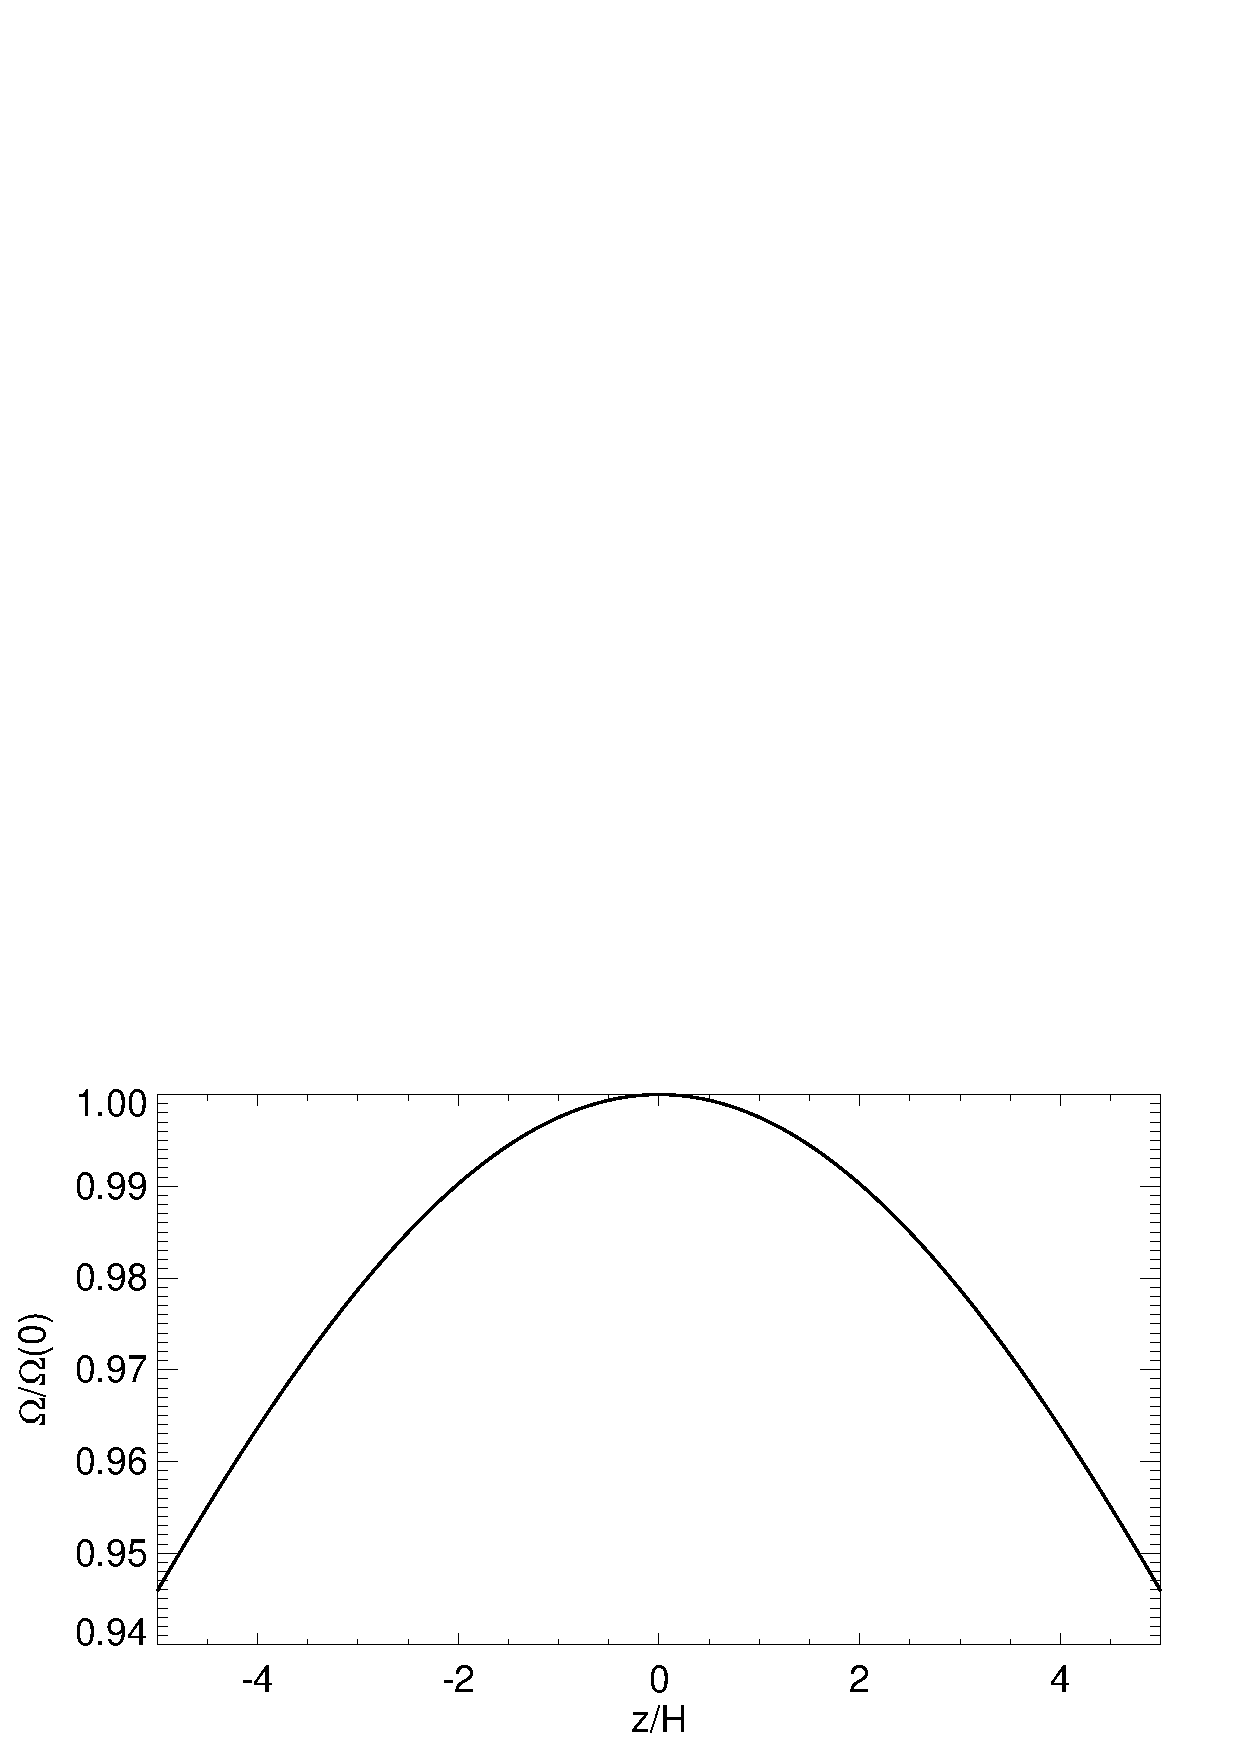
\includegraphics[width=\linewidth,clip=true,trim=0cm 0cm 0cm
  0cm]{figures/omega2} 
  \caption{Equilibrium rotation profile $\Omega(z)$,
    normalized by its mid-plane value, for  the fiducial disk model with $\Gamma=1.011$
    and $(p,q, h)=(-1.5,-1,0.05)$. 
    \label{omega_z} 
  }
\end{figure}

\subsection{VSI with rapid thermal relaxation}\label{vertiso_pertiso} 
We first calculate the VSI in a disk with rapid thermal relaxation by
setting $\beta=10^{-3}$. (Smaller values yield similar results.) 
This setup mimics strictly isothermal perturbations in a vertically
isothermal disk, already considered previously \citepalias{nelson13,mcnally14,barker15}. 
For completeness, and as a way of introducing terminology, 
we review this case before considering the effect of 
thermal relaxation. %A more detailed analysis is given by \cite{barker15}.   

% Fig. \ref{iso_eigen_kx} compares the numerically obtained eigenvalues 
% for the fundamental mode and that calculated from 
% Eq. \ref{simple_growth}. We find good agreement in the
% wave frequency $\omega$ at all $\khat$ and in growth rates $\nu$ for
% $\khat\gtrsim 10$. Growth rates are over-estimated by our analysis but 
% are $O( h\Omega_k)$, which is consistent with the discussion in
% Appendix \ref{max_growth1}. The match in $\nu$ worsens for 
% decreasing $\khat$ due to the neglect of global radial structure in
% the analysis. Nevertheless, given the number of approximations made
% in our analysis, the agreement is satisfactory. 

% \begin{figure}
%   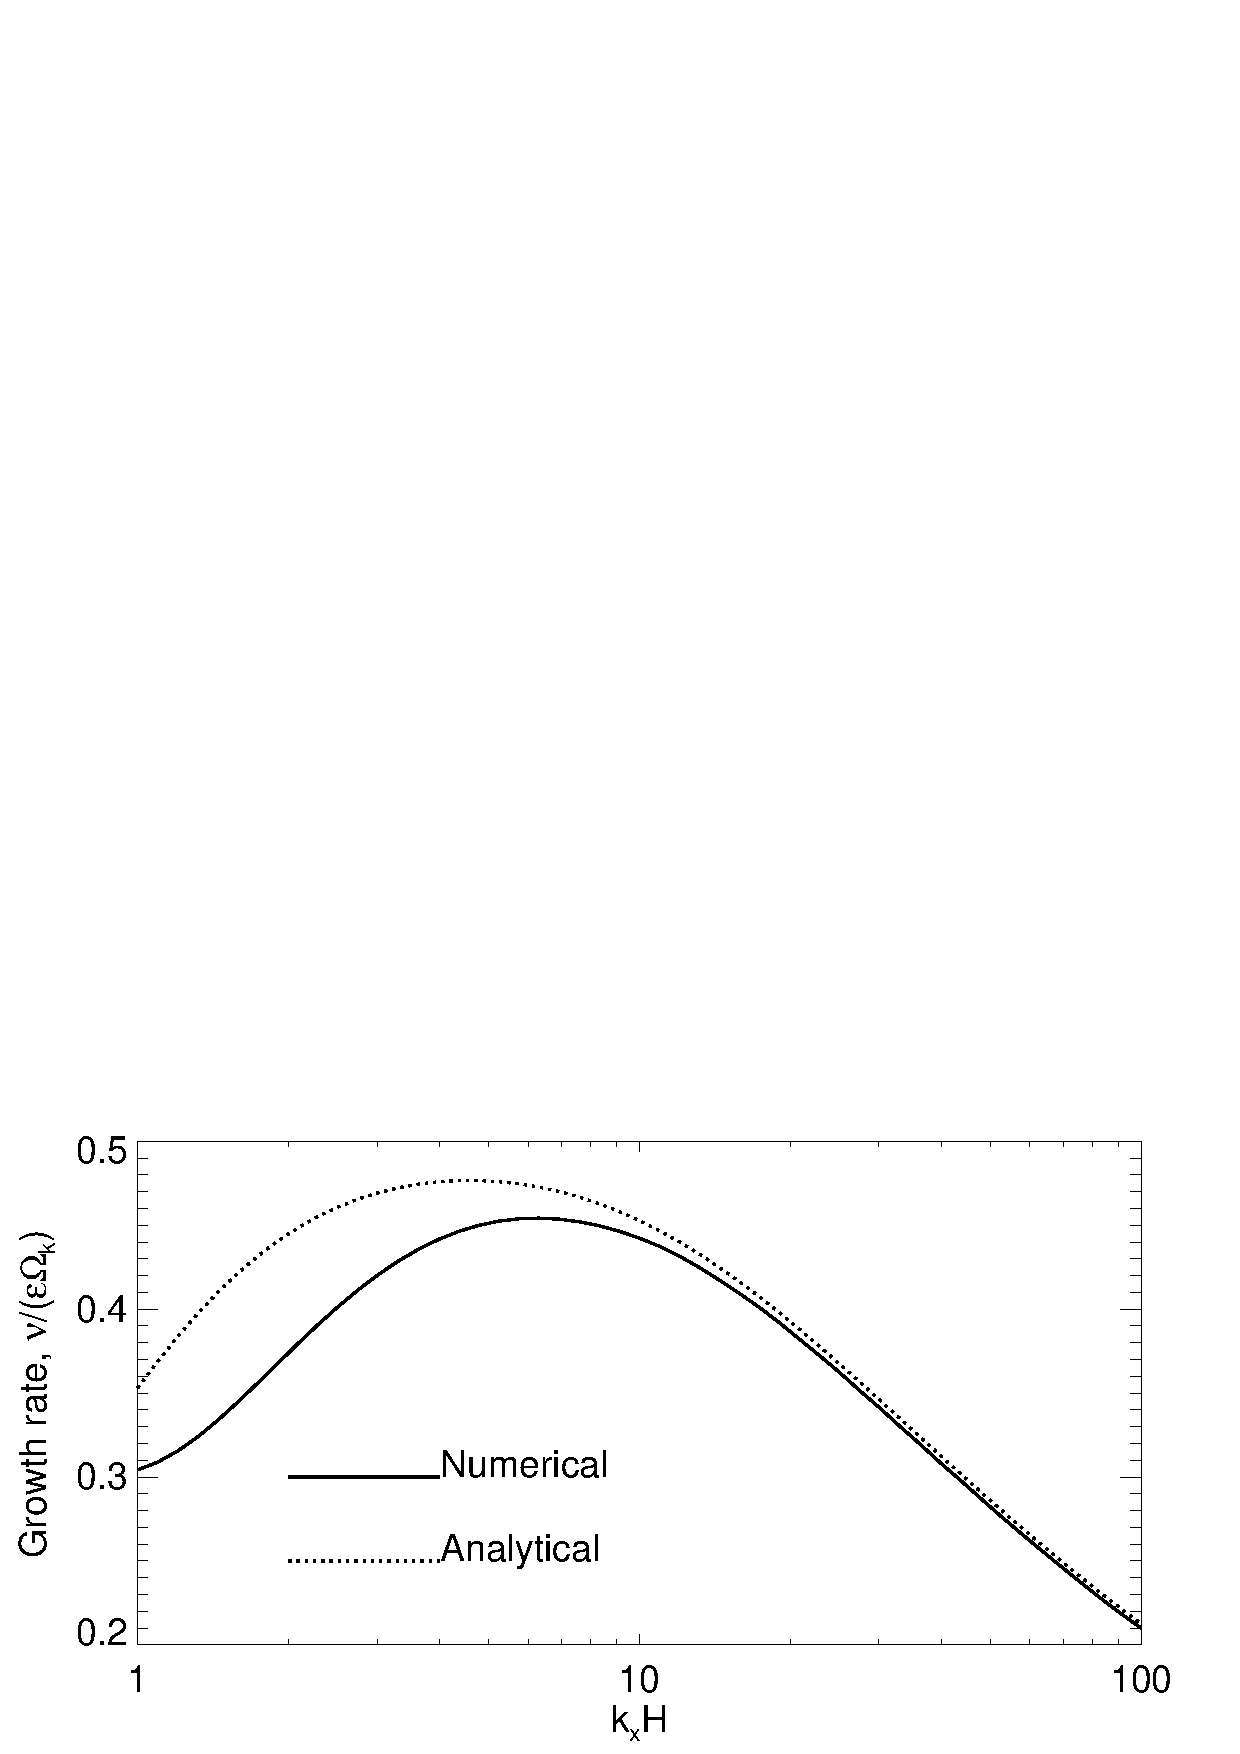
\includegraphics[width=\linewidth,clip=true,trim=0cm 1.75cm 0cm
%   0cm]{figures/compare_eigen_imag_iso} 
%   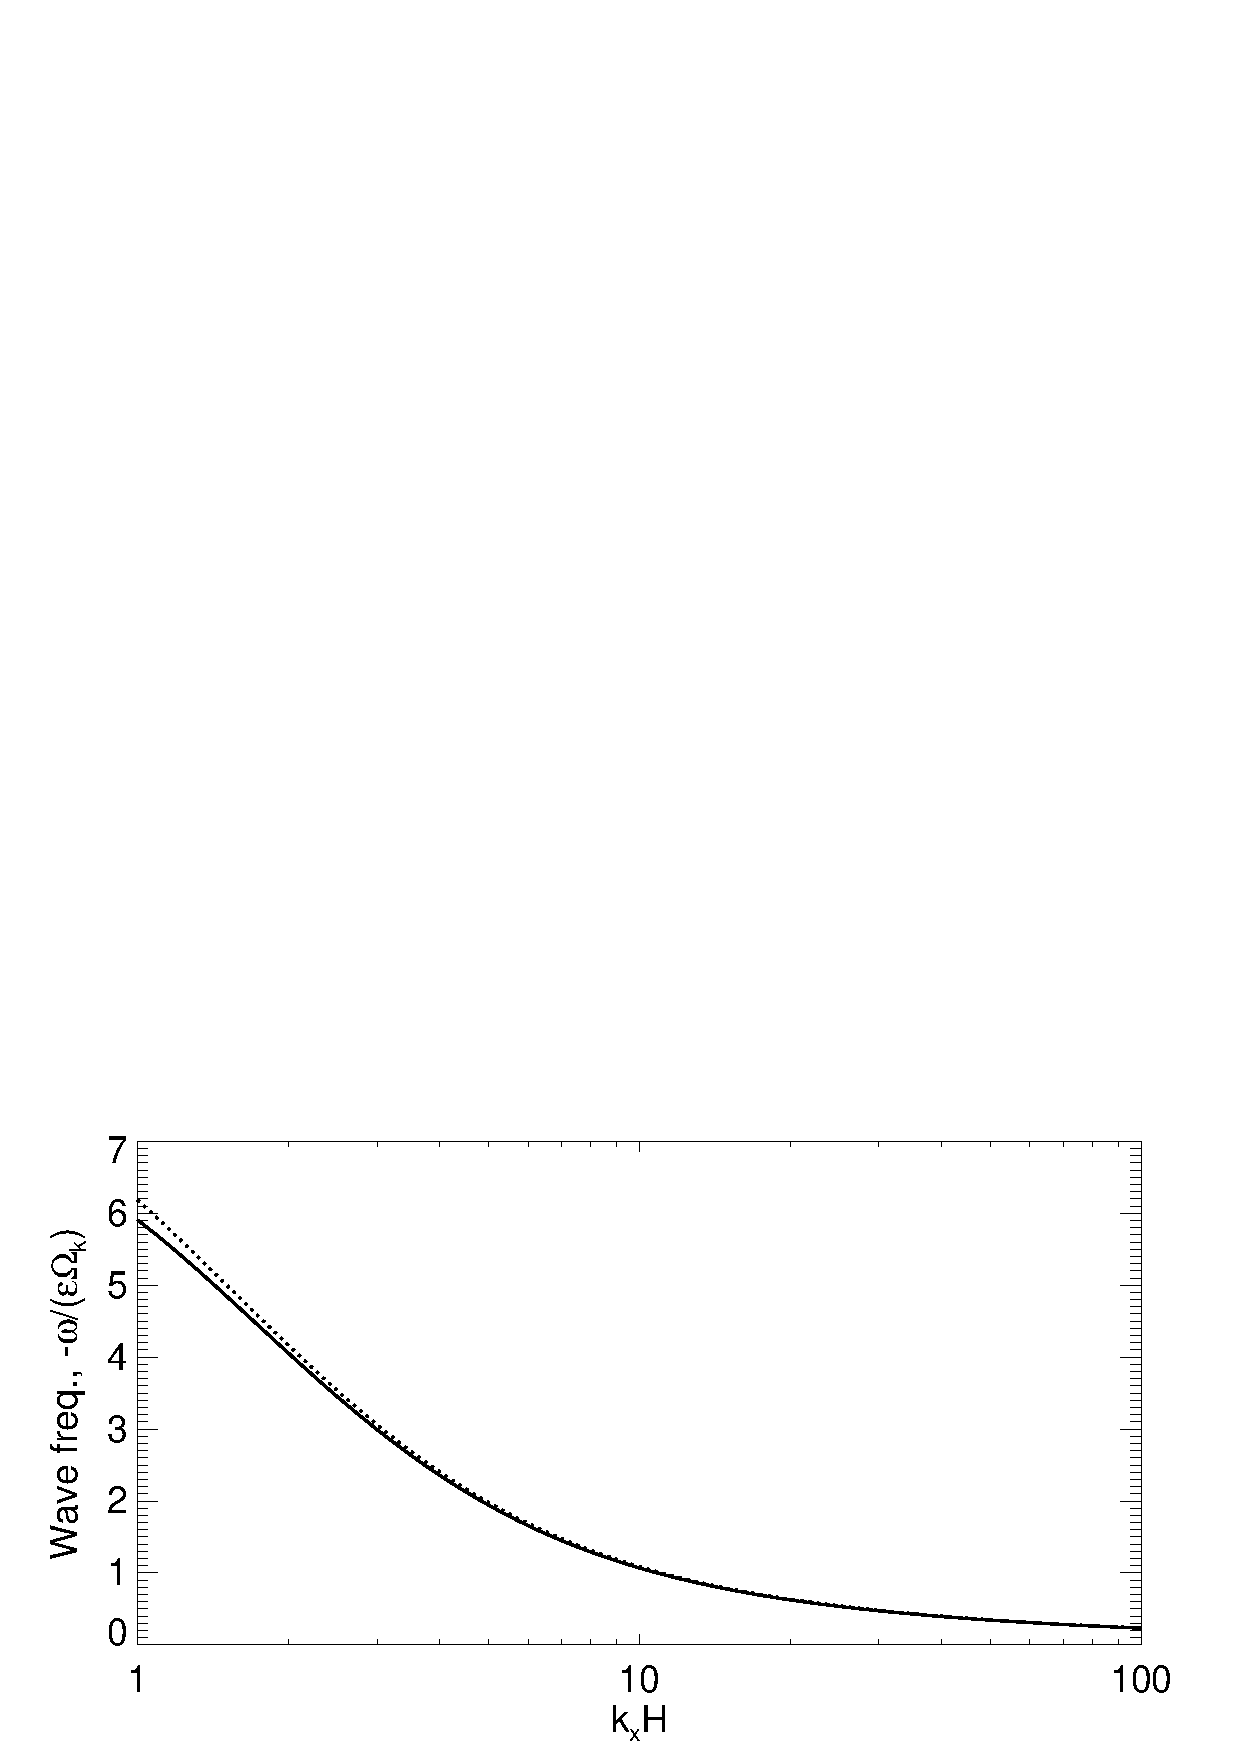
\includegraphics[width=\linewidth,clip=true,trim=0cm 0cm 0cm
%   1cm]{figures/compare_eigen_real_iso}
%   \caption{Growth rate (top) and real frequency (bottom) of the
%     fundamental VSI mode in the fiducial disk model with $\beta =
%     10^{-3}$. 
%     % a disk with $(\gamma,
%     % \Gamma)=(1.4,1.011)$, $(p,q, h)=(-1.5,-1,0.1)$ and
%     % $\beta=10^{-3}$. 
%     The solid (dotted) line is obtained numerically
%     (analytically).  
%     \label{iso_eigen_kx} 
%   }
% \end{figure}

% With rapid thermal relaxation, growth rates are expected to diminish
% for both $\khat\to 0$ and $\khat\to \infty$. This is because for
% $\khat\ll 1$ the radial wavelength is large, but such disturbances are 
% stabilized by by epicyclic motions ($|\omega|\sim
% \kappa$). Disturbances with $\khat\gg 1$ are radially localized, but  
% there is no energy change when fluid elements are perturbed at fixed
% cylindrical radius whilst conserving its angular momentum (applicable
% to axisymmetric perturbations).

\subsubsection{Case study: $\khat=10$}
In Fig. \ref{compare_modes_iso_kx10} we plot eigenvalues of unstable 
modes with $\khat=10$. Black dots correspond to our fiducial setup.  
We also plot results obtained with different 
vertical boundary conditions: rigid boundary and $\zmax=5H$ (red
crosses),  free surface and $\zmax = 3H$ (blue triangles), free surface
and $\zmax=7H$ (green crosses). 

The modes shown in Fig. \ref{compare_modes_iso_kx10} are `body modes'
and are inertial waves destabilized by vertical shear
\citepalias{barker15}. (The exception being the fastest growing
mode for $\zmax=7H$ which is a surface mode --- see the discussion
below.)  The `fundamental corrugation mode', marked by `f',
corresponds to the eigenvalue with the smallest $|\sigma|$. The
fundamental mode is robust  
against vertical boundary conditions as it appears at the same
position in Fig. \ref{compare_modes_iso_kx10} for all cases. Higher  
order modes, corresponding to increasing $|\omega|$, increasingly
deviates from the analytic line due to the imposed boundaries, 
unless $\zmax$ is increased. 

\begin{figure}
  \includegraphics[width=\linewidth]{figures/compare_modes_iso_kx10_analytic.ps}
  \caption{Unstable modes with $\khat=10$ in the fiducial disk model
    with $\beta=10^{-3}$. %  a disk with 
    % $(\gamma,\Gamma)=(1.4,1.011)$, $(p,q, h)=(-1.5,-1,0.1)$ and
    % $\beta=10^{-3}$. 
    The fiducial boundary condition is a free surface ($\Delta P=0$)
    with vertical domain size $\zmax=5H$  (black dots).  Other
    cases correspond to different boundary conditions applied at
    different heights. The fundamental mode is marked by `f'. Lines
    are computed from the analytic dispersion relation 
    with thermal relaxation Eq. \ref{relax_disp} (dotted), and that for
    isothermal perturbations, Eq. \ref{simple_growth} (dashed). 
    \label{compare_modes_iso_kx10} 
  }
\end{figure}

For later comparison, we plot in Fig. \ref{lowfreq_eigenfunc} the 
eigenfunctions $W$ and $\delta   v_z$ for the fundamental mode. We also show a 
meridional visualization in Fig. \ref{lowfreq_eigenfunc_2d}. The $x$ axis is 
stretched for clarity; radial velocities are in fact typically much 
smaller than vertical velocities. Most of the meridional kinetic energy is
contained within $\sim 2H$ of the midplane due to the density 
stratification. 

\begin{figure}
  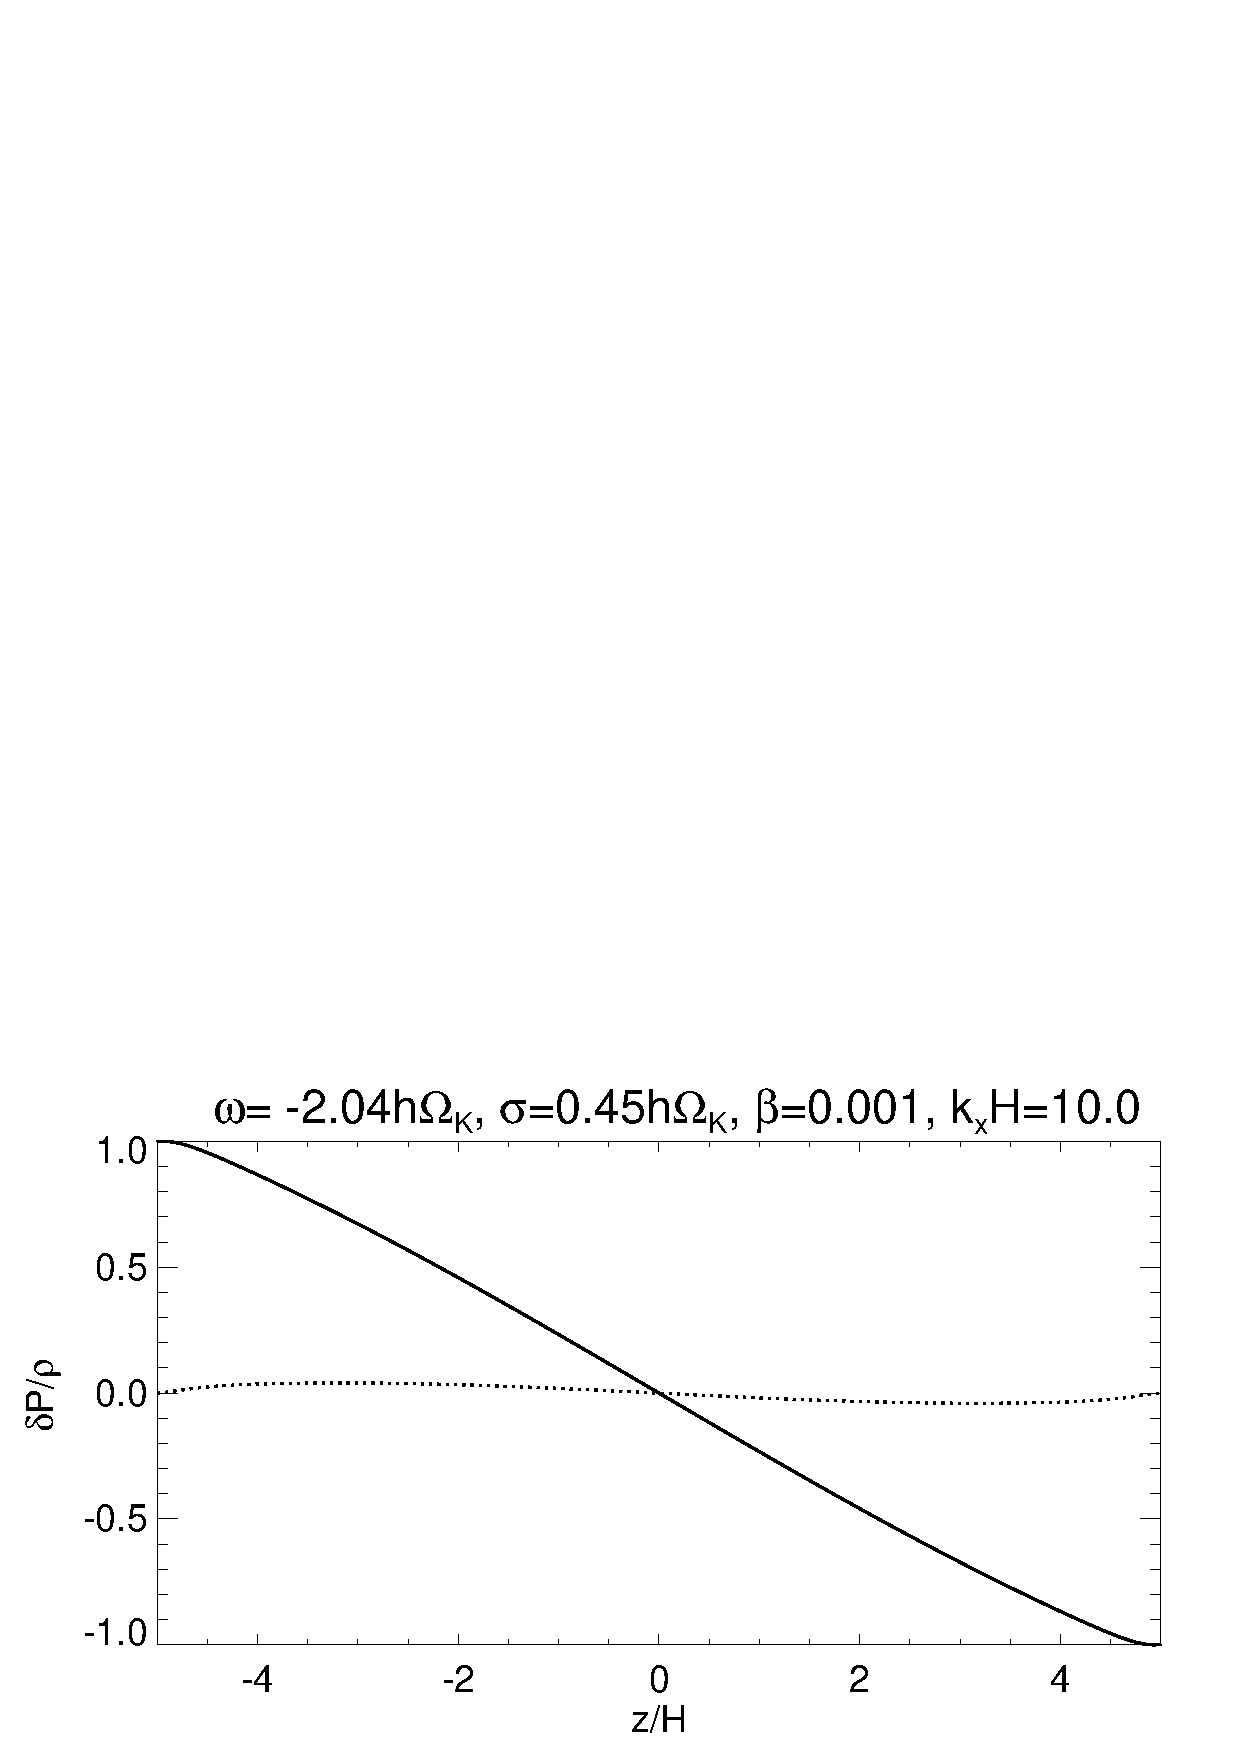
\includegraphics[width=\linewidth,clip=true,trim=0cm 1.75cm 0cm
  0cm]{figures/eigenvectorW_iso} 
  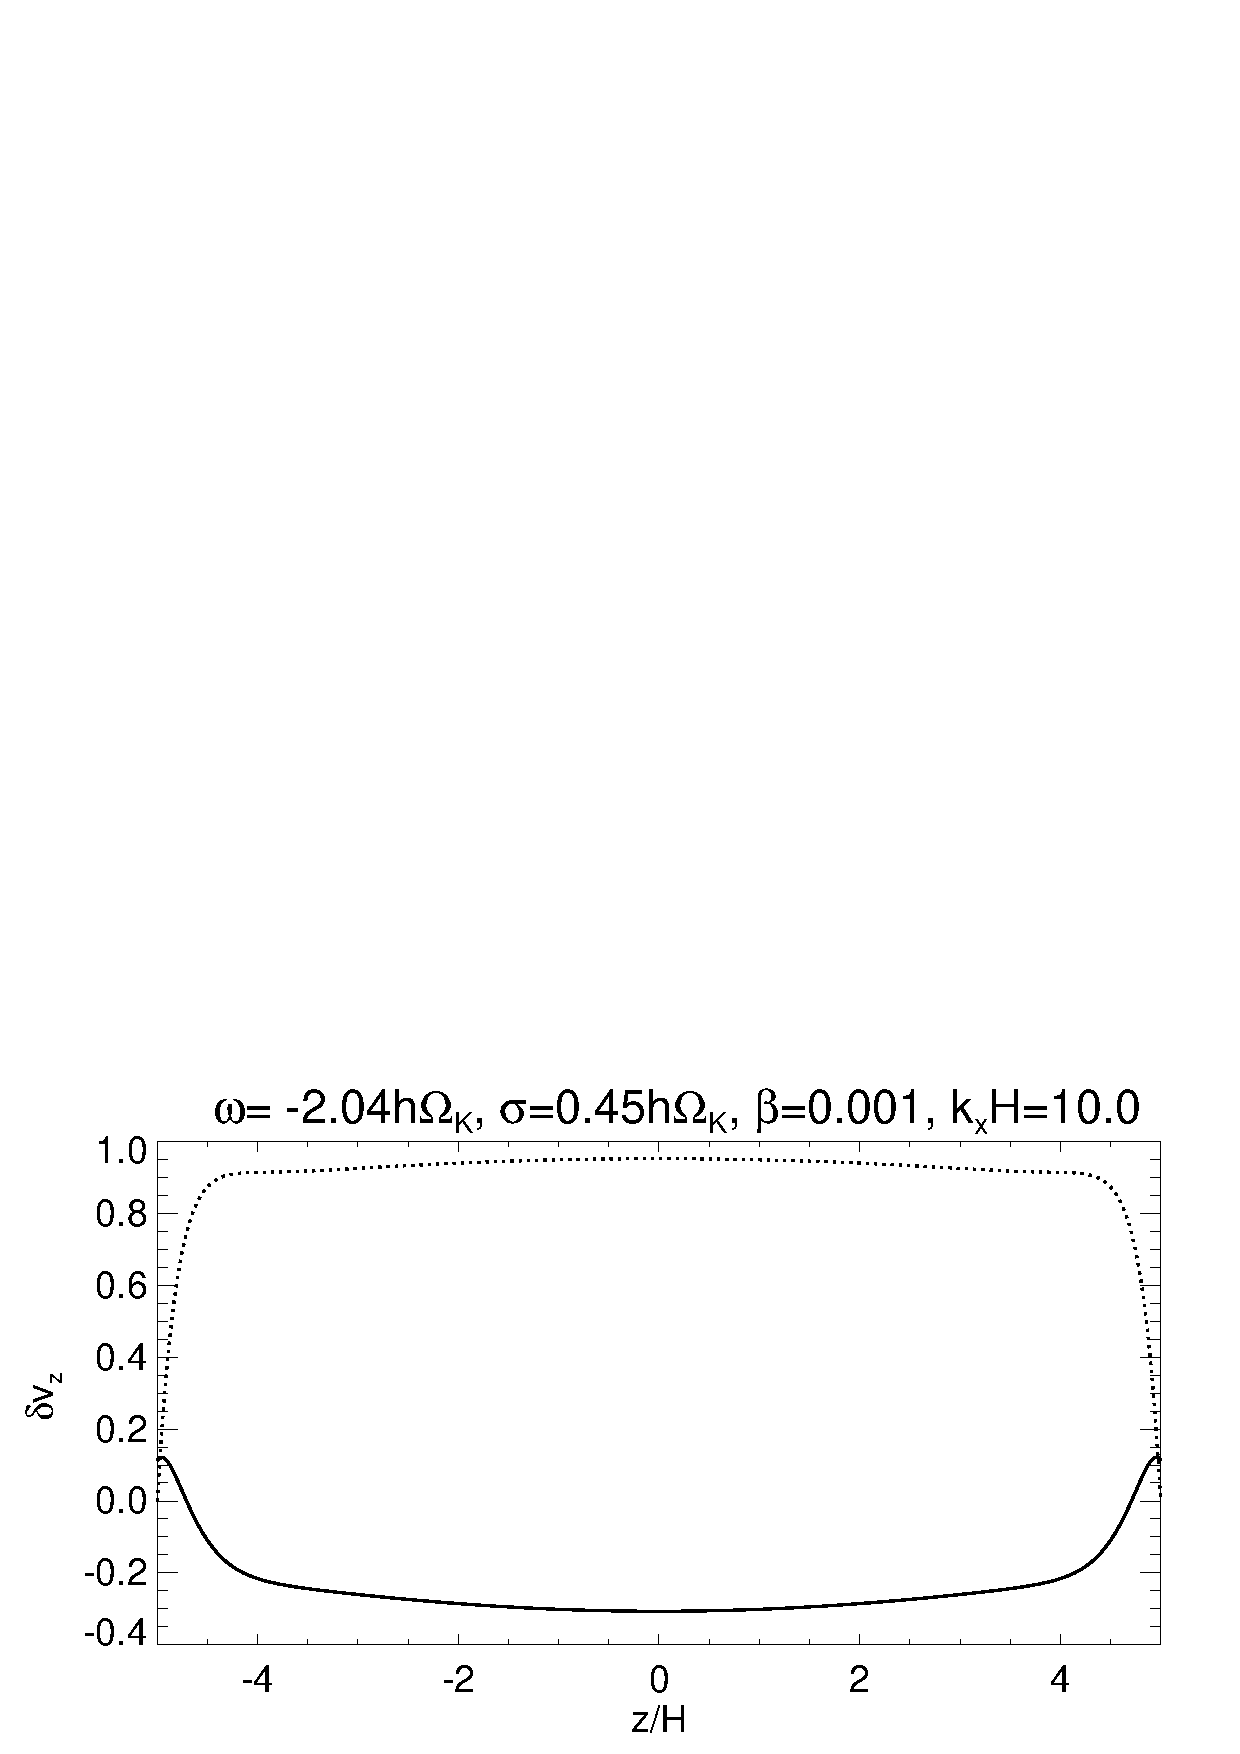
\includegraphics[width=\linewidth,clip=true,trim=0cm 0cm 0cm
  1cm]{figures/eigenvectorvz_iso}
  \caption{Pseudo-enthalpy perturbation $W$ (top) and vertical velocity
    perturbation $\delta v_z$ of the fundamental VSI with 
    $\khat=10$ in the fiducial disk with rapid thermal relaxation $\beta=10^{-3}$. The real  
    (imaginary) parts of $W$ and $\delta v_z$ are plotted as solid 
    (dotted) lines.  
    \label{lowfreq_eigenfunc}
  }
\end{figure}

\begin{figure}
%  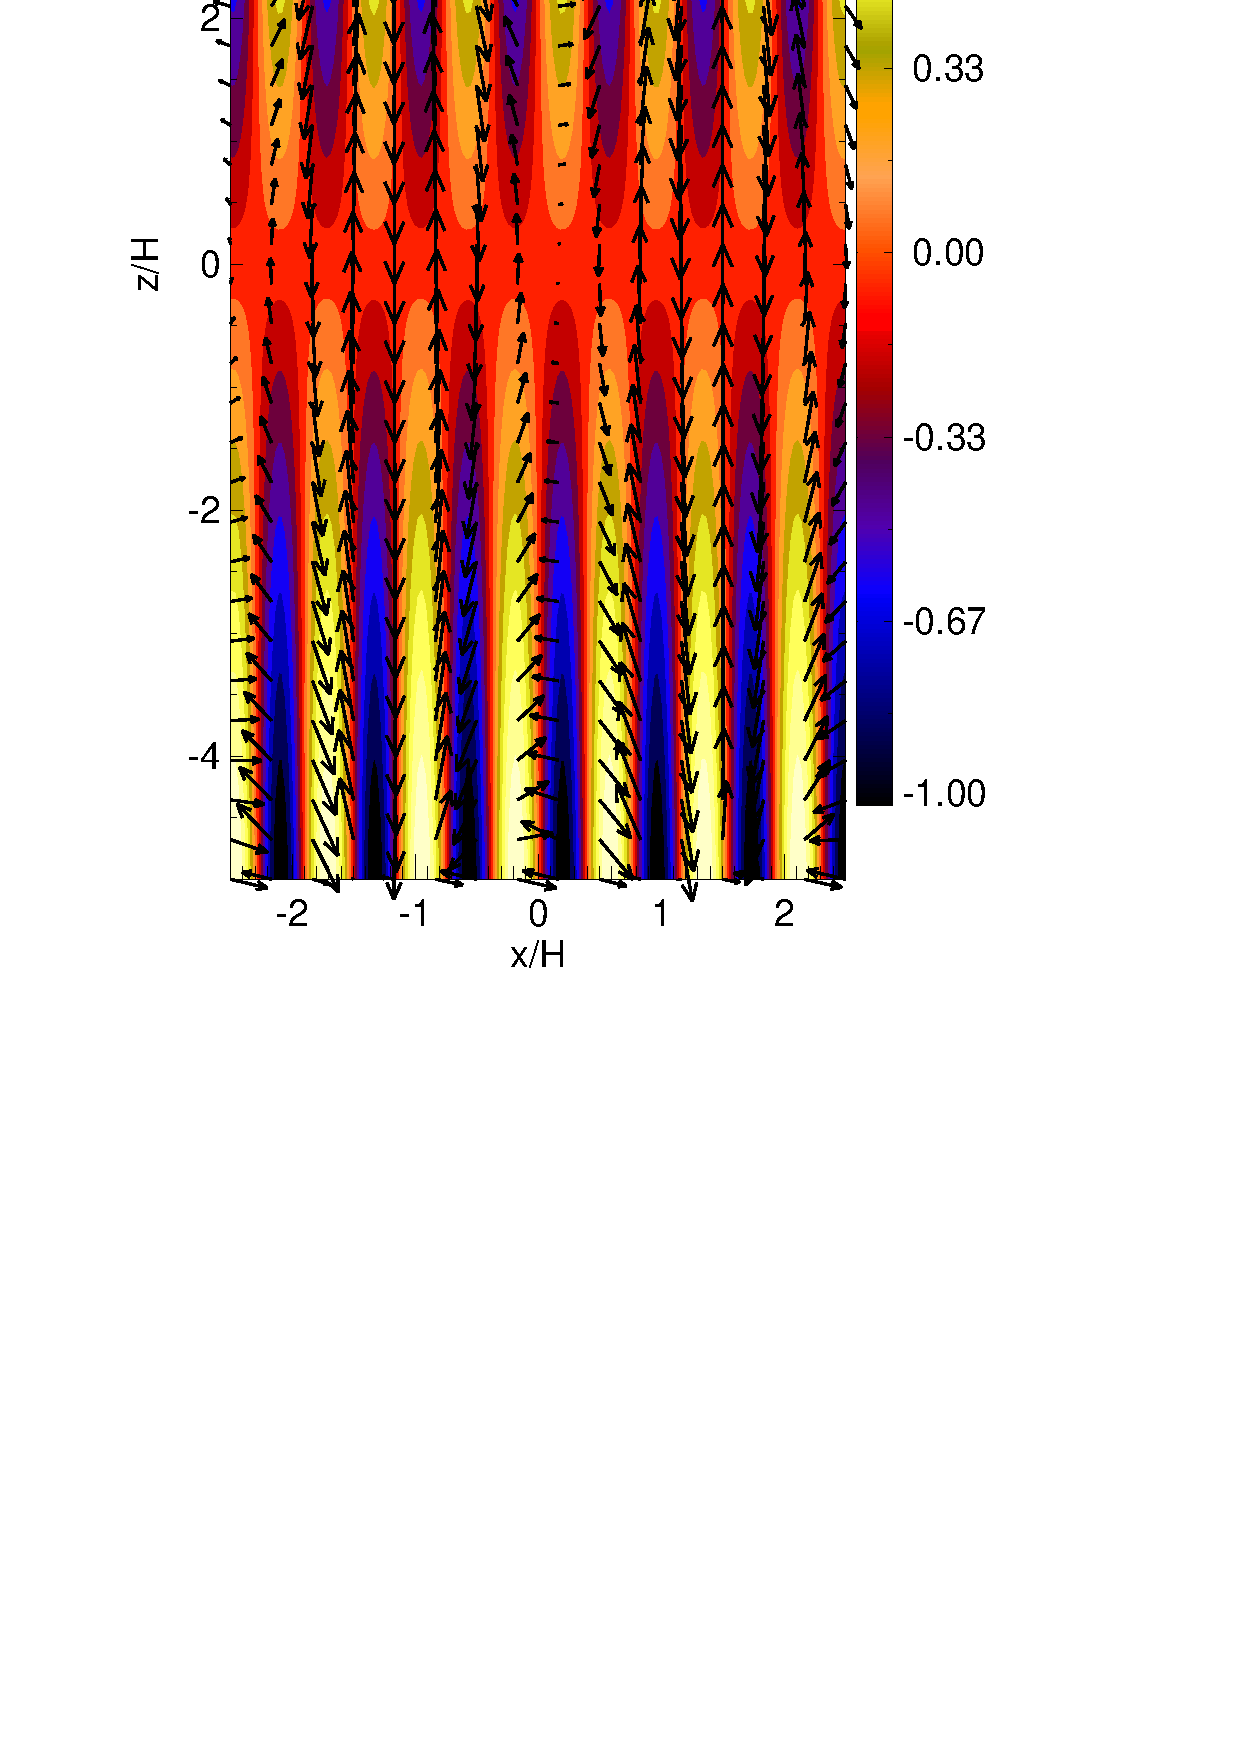
\includegraphics[scale=0.345,clip=true,trim=0cm 0cm 2.5cm
%  0cm]{figures/result2d_vel}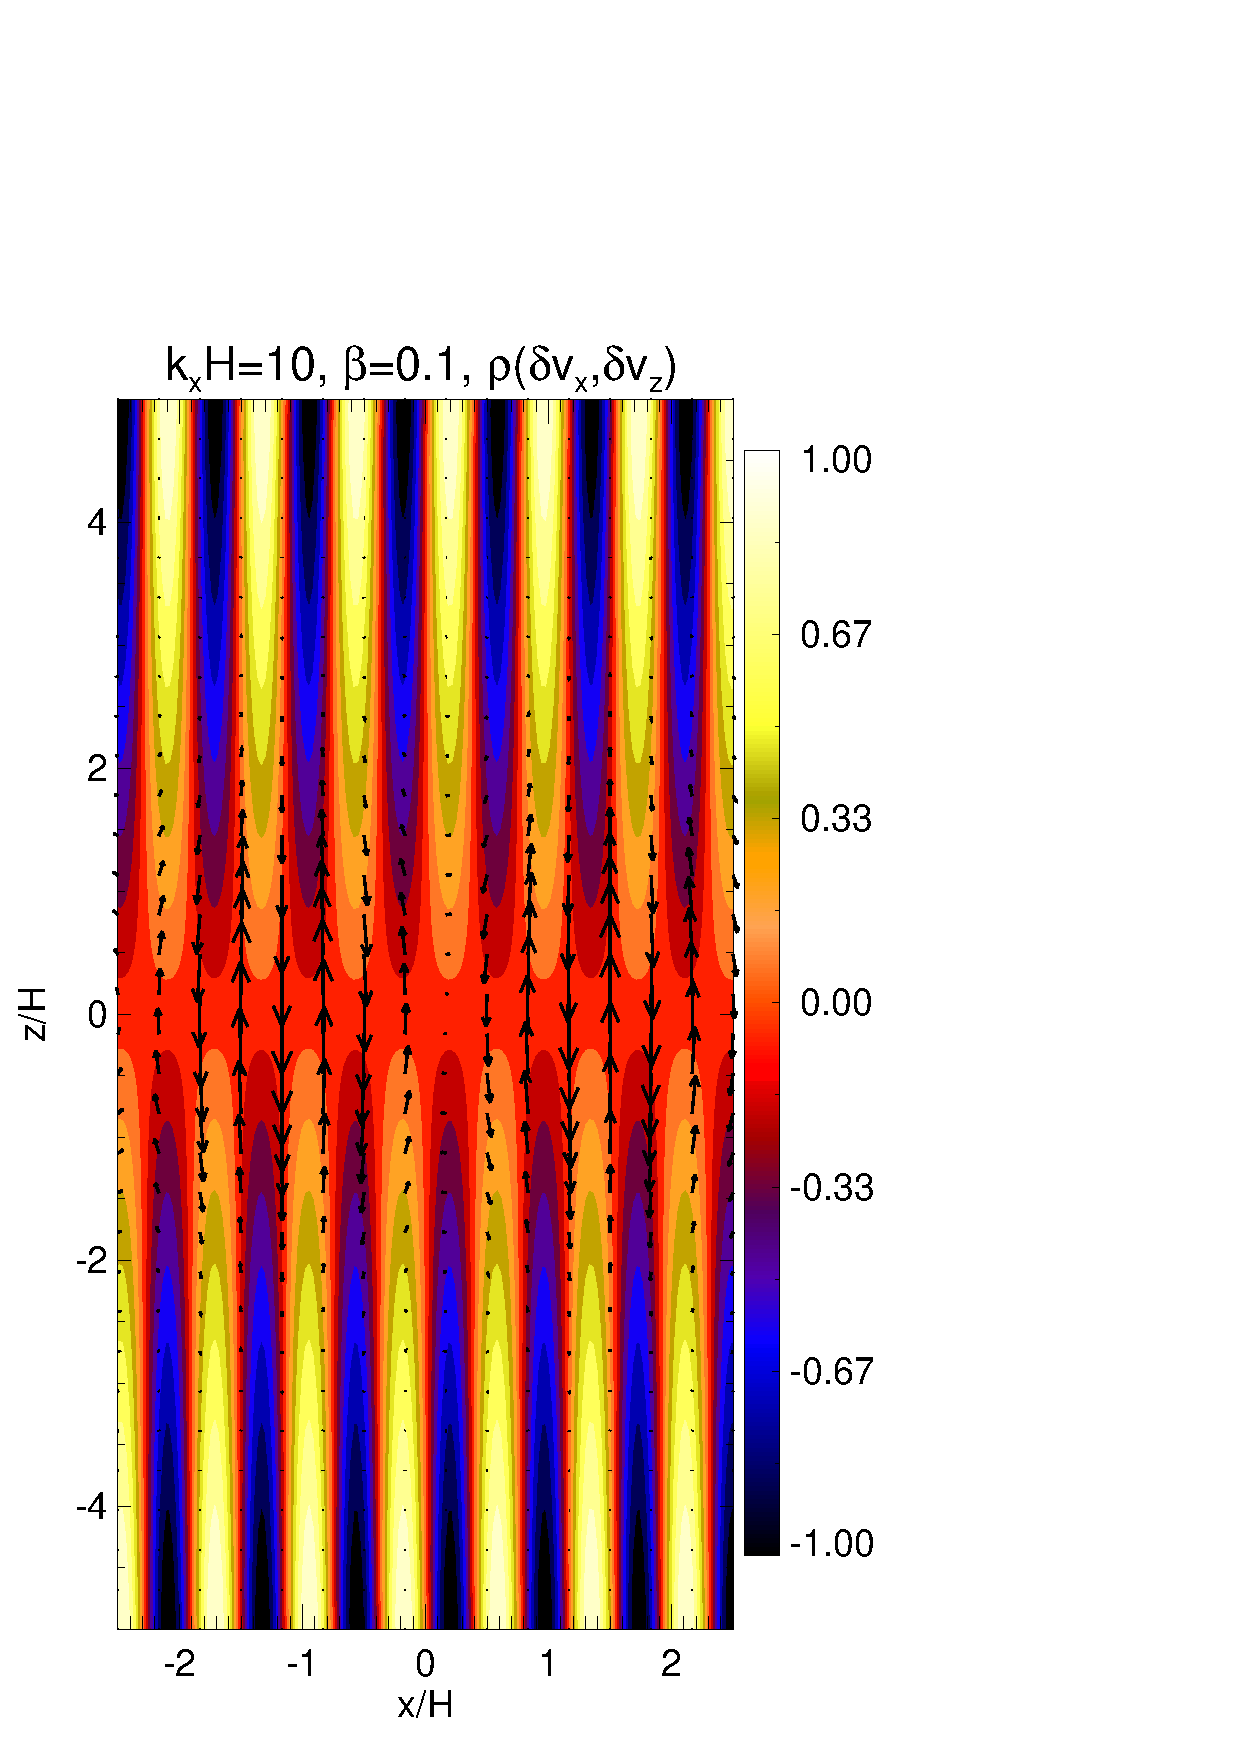
\includegraphics[scale=0.345,clip=true,trim=1.9cm 0cm 0cm
%  0cm]{figures/result2d_mom} 
  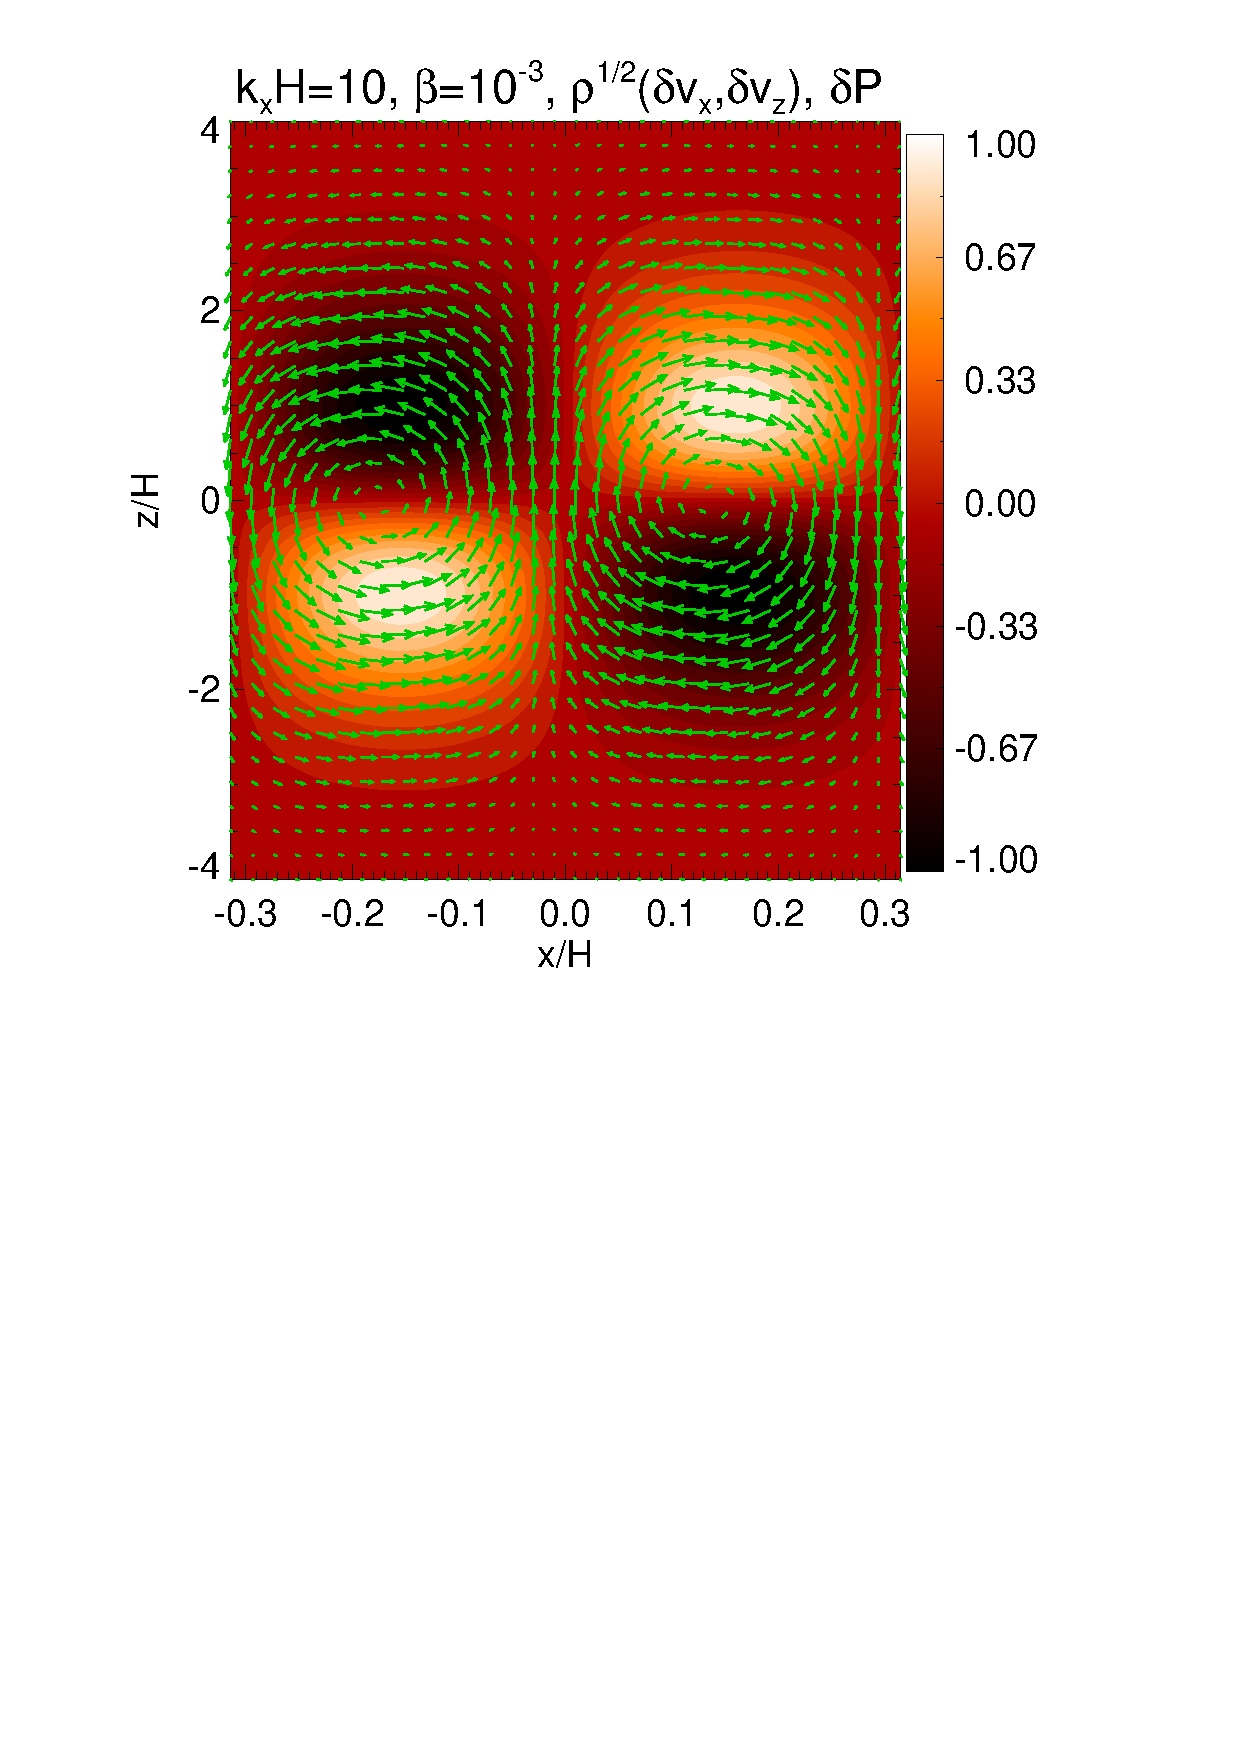
\includegraphics[width=\linewidth]{figures/result2d_iso}
  \caption{Visualization of the fundamental VSI mode in
    Fig. \ref{lowfreq_eigenfunc}. The color scale corresponds to the
    pressure perturbation $\delta P=\rho W$ scaled by its maximum value.
    Arrows correspond to the vector field field $\sqrt{\rho}(\delta
    v_x,\delta v_z)$. Note that the horizontal axis has been stretched 
    for clarity.  
    \label{lowfreq_eigenfunc_2d}
  }
\end{figure}

\subsubsection{Comment on `surface modes'}\label{surf_comment} 
Fig. \ref{compare_modes_iso_kx10} lack the distinct `surface modes' found by 
\citetalias{nelson13}, \citetalias{mcnally14}  and \citetalias{barker15}. 
This a class of unstable modes associated with vertical shear near the
disk boundaries. They are absent in our  
analysis because there we assumed a disk with infinite 
vertical extent, since the vertically isothermal disk has no
surface. However, surface modes can occur in the present calculations 
because there is an imposed vertical boundary.   

We illustrate surface modes in Fig. \ref{compare_modes_iso_kx30} 
which show unstable modes with $\khat=30$. Surface 
modes lie almost parallel to the vertical axis 
in such diagrams. They are readily identified for  $\zmax\geq 5H$ and
are marked by `s'.  Fig. \ref{lowfreq_eigenfunc_surf} shows an example
of a surface mode. We typically find an increasing
number of surface modes with increasing $\zmax$ and/or $\khat$. 
%consistent with \cite{barker15}. 
 
As explained by \citetalias{barker15}, while surface modes have a physical
origin, their occurence in the vertically isothermal disk is due to
imposing a finite vertical domain size. This has important
implications when interpreting results obtained from the vertically
isothermal disk model. For example, seeking the most unstable mode may
result in a surface mode, but its growth rate would depend on
$\zmax$. We return to this issue later.     

%Thus, the
%vertically isothermal disk is not useful for studying surface modes. 
%Thus, seeking the most unstable mode in a vertically isothermal disk
%may not yield robust results because this 

\begin{figure}
  \includegraphics[width=\linewidth]{figures/compare_modes_iso_kx30_analytic.ps}
  \caption{Same as Fig. \ref{compare_modes_iso_kx10} but for
    $\khat=30$. Examples of surface modes are 
    marked by `s'. \label{compare_modes_iso_kx30}
  }
\end{figure}


\begin{figure}
  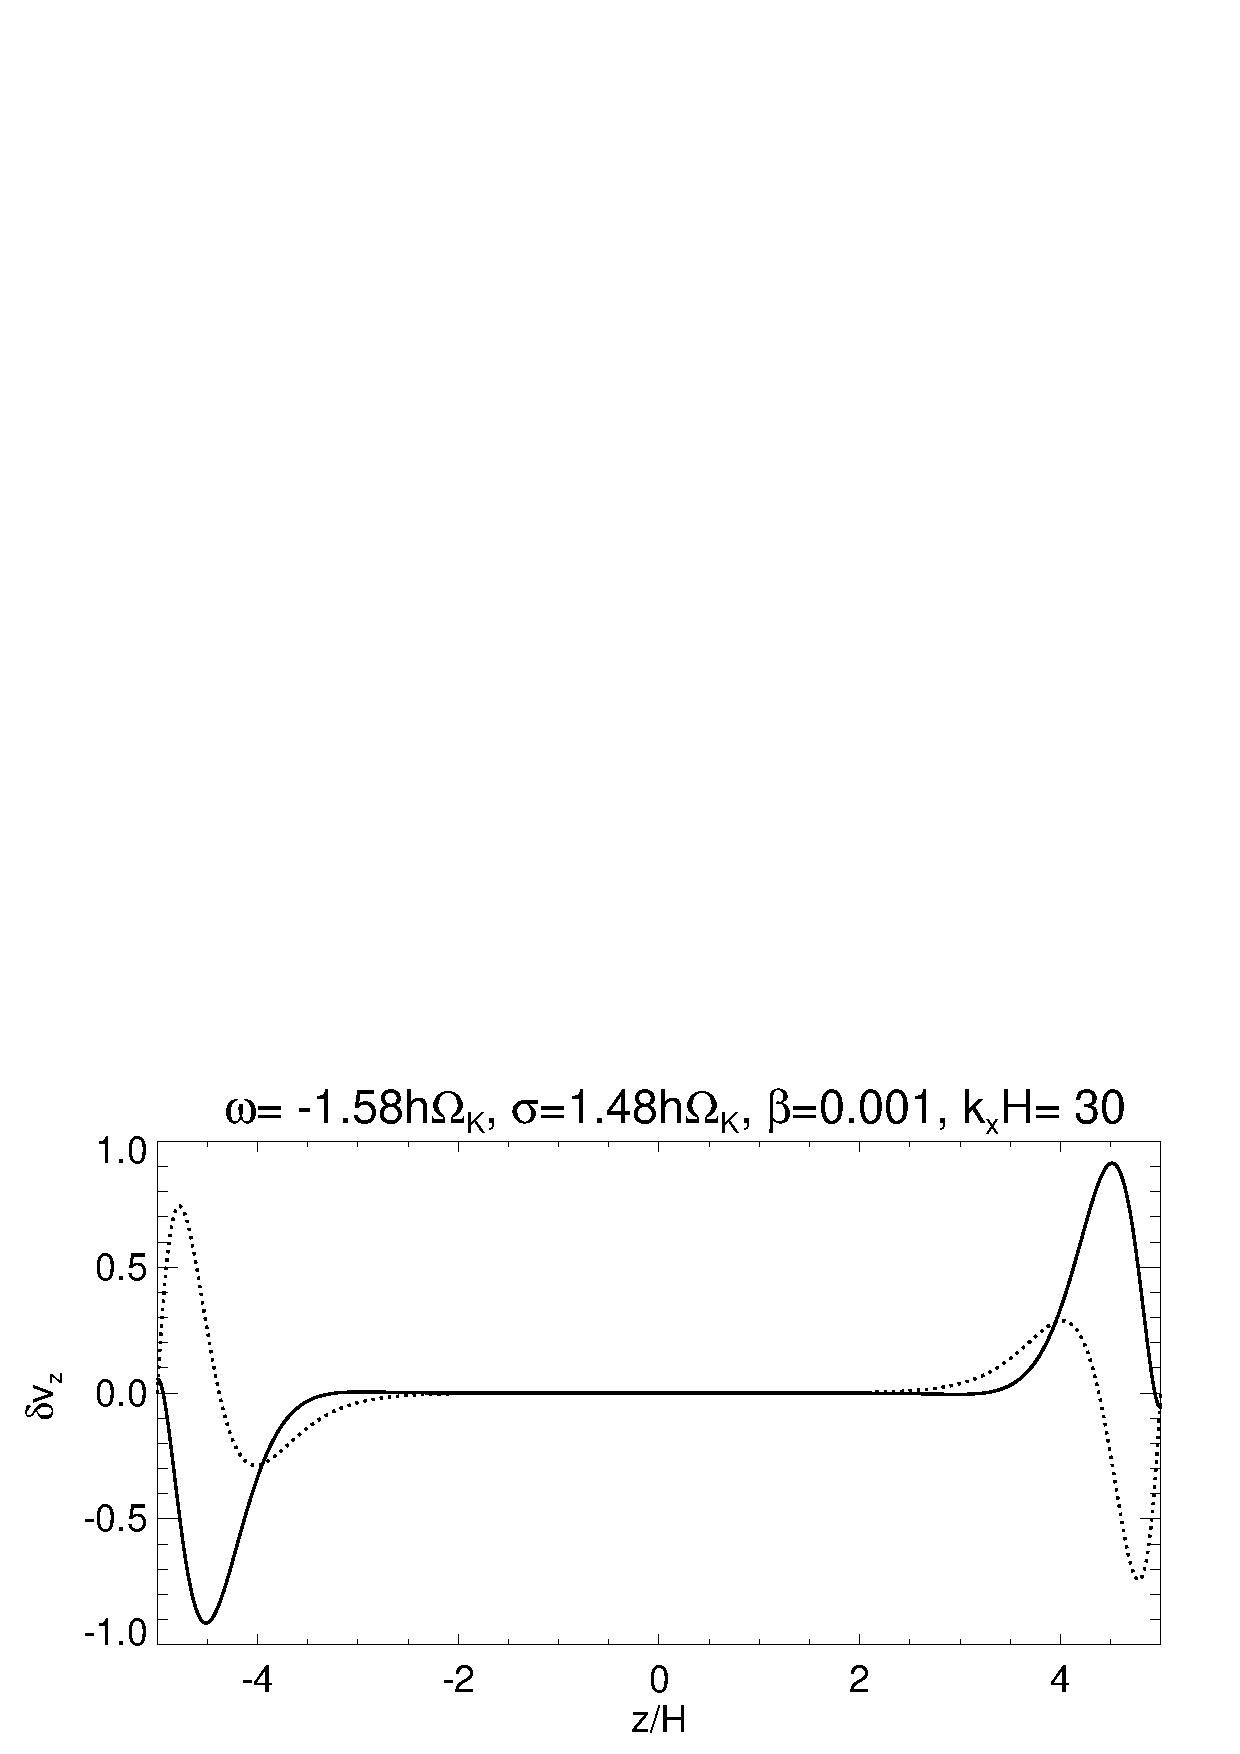
\includegraphics[width=\linewidth,clip=true,trim=0cm 0cm 0cm
  0cm]{figures/eigenvectorvz_iso_surf}
  \caption{Example of a `surface mode' in the fiducial disk model.
    \label{lowfreq_eigenfunc_surf}
  }
\end{figure}

\subsection{Effect of thermal relaxation}\label{therm_relax_eff}
We now consider the effect of finite thermal relaxation by increasing 
$\beta$. % Note that for the fiducial disk model the critical thermal 
% timescale $\beta_\mathrm{crit} = 0.125$.
Fig. \ref{compare_modes_cool_kx10} show unstable modes with $\khat=10$ 
and $\beta\in[0.01,0.1]$. In addition to our fiducial setup with 
$\zmax=5H$, we also plot results for $\zmax=3H$, $\zmax=7H$ and 
analytic results computed from Eq. \ref{relax_disp}.  %analytic
% results for low order modes 

We find the number of unstable modes decrease with increasing
$\beta$. Consider the fiducial setup with $\zmax=5H$ 
(middle panel). The fundamental mode ($M=0$) is not the most unstable for   
$\beta=0.01$ as there area number of modes with $M>0$ that have larger
growth rates. As noted above, these higher order modes are affected by
$\zmax$, e.g. there is a significant mismatch between numerical and 
analytical results for $M\geq1$ when $\zmax=3H$ (upper panel). 

%However, by comparing with results for $\zmax=3H$, we see that 

However, the fundamental mode becomes dominant for $\beta \geq 
0.03$. Higher order modes, which would be dominant at small $\beta$, 
are more effectively stabilized with increasing $\beta$. For 
$\beta=0.1$, which is close to the critical thermal timescale
$\beta_\mathrm{crit} (=0.125$ for the fiducial disk
parameters), we only find the fundamental mode. This is consistent with
the discussion in \S\ref{iso_vsi_beta_crit}.    

\begin{figure}
  \includegraphics[width=\linewidth,clip=true,trim=0cm 1.75cm 0cm
  0cm]{figures/compare_modes_cool_kx10_z3_analytic.ps} 
  \includegraphics[width=\linewidth,clip=true,trim=0cm 1.75cm 0cm
  0cm]{figures/compare_modes_cool_kx10_z5_analytic.ps}
  \includegraphics[width=\linewidth]{figures/compare_modes_cool_kx10_z7_analytic.ps}
  \caption{Unstable modes with $\khat=10$ and thermal
    relaxation timescales $\beta=0.01$ (black dots), $\beta=0.03$ (red
    crosses), $\beta=0.05$ (blue triangles) and $\beta=0.1$ (green 
    crosses); for different vertical domain sizes $\zmax=3H$ (top),
    $\zmax=5H$ (middle, the fiducial setup) and $\zmax=7H$
    (bottom). Lines are computed from
    Eq. \ref{relax_disp} for  $M=0$ (solid, fundamental mode) and
    $M=1,\,2,\,3$ (dotted, dashed, dash-dot, respectively). Along each
    line, $\beta$ increases continuously from $0.01$ to $0.1$ from top
    to bottom, and squares mark corresponding $\beta$ values with
    numerical results. 
    \label{compare_modes_cool_kx10} 
  }
\end{figure}

Fig. \ref{lowfreq_eigenfunc_cool}---\ref{lowfreq_eigenfunc_2d_cool}
shows the fundamental mode with $\khat=10$ in a disk with 
$\beta=0.1$. Comparing these plots with
Fig. \ref{lowfreq_eigenfunc}---\ref{lowfreq_eigenfunc_2d}, which have
$\beta=10^{-3}$, we see that increasing $\beta$ restricts the region 
characterized by $W\sim z$ and $\delta v_z\sim$ constant closer to the
midplane, with oscillatory behavior emerging near vertical boundaries
where buoyancy first becomes important. This leads to the `tilted'
pressure perturbations seen in Fig. \ref{lowfreq_eigenfunc_2d_cool} 
(cf. Fig. \ref{lowfreq_eigenfunc_2d}). 

\begin{figure}
  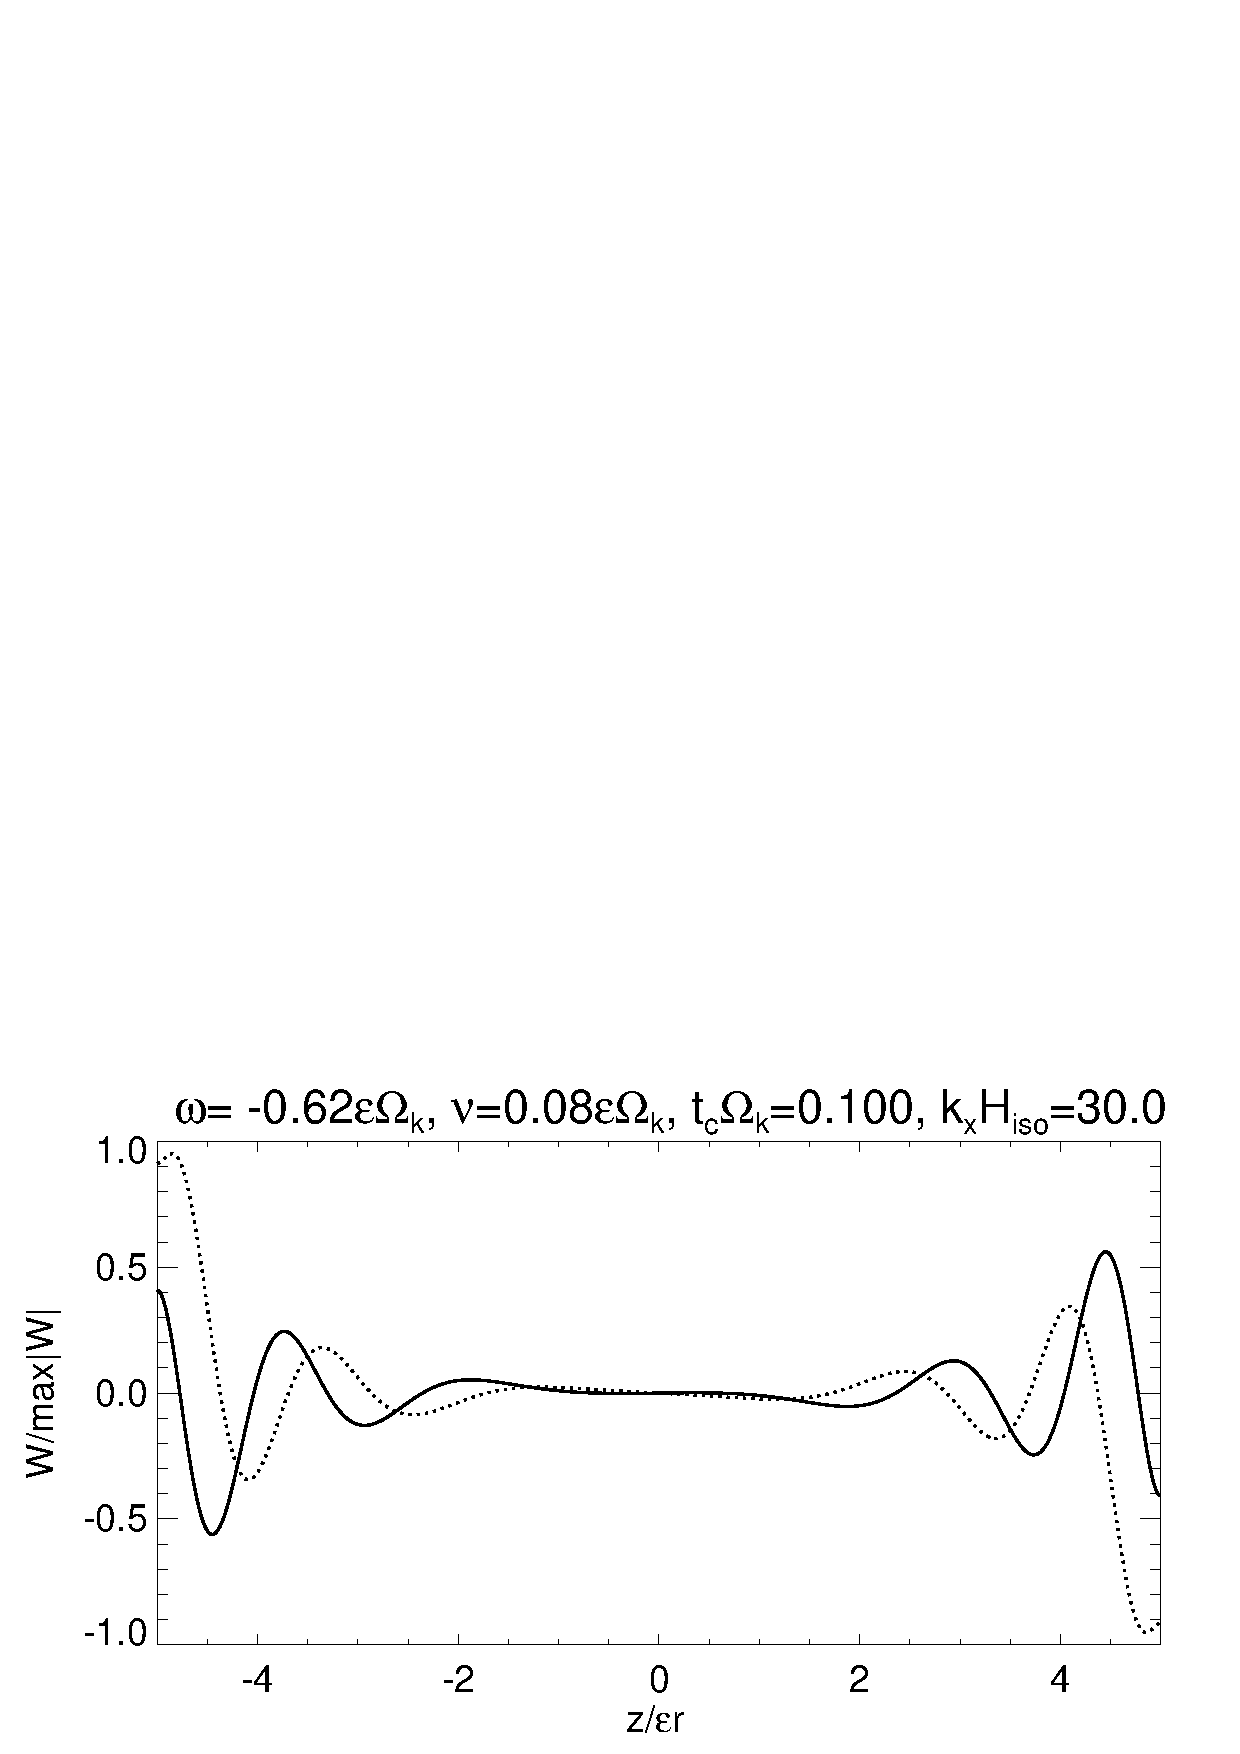
\includegraphics[width=\linewidth,clip=true,trim=0cm 1.75cm 0cm
  0cm]{figures/eigenvectorW_beta0d1} 
  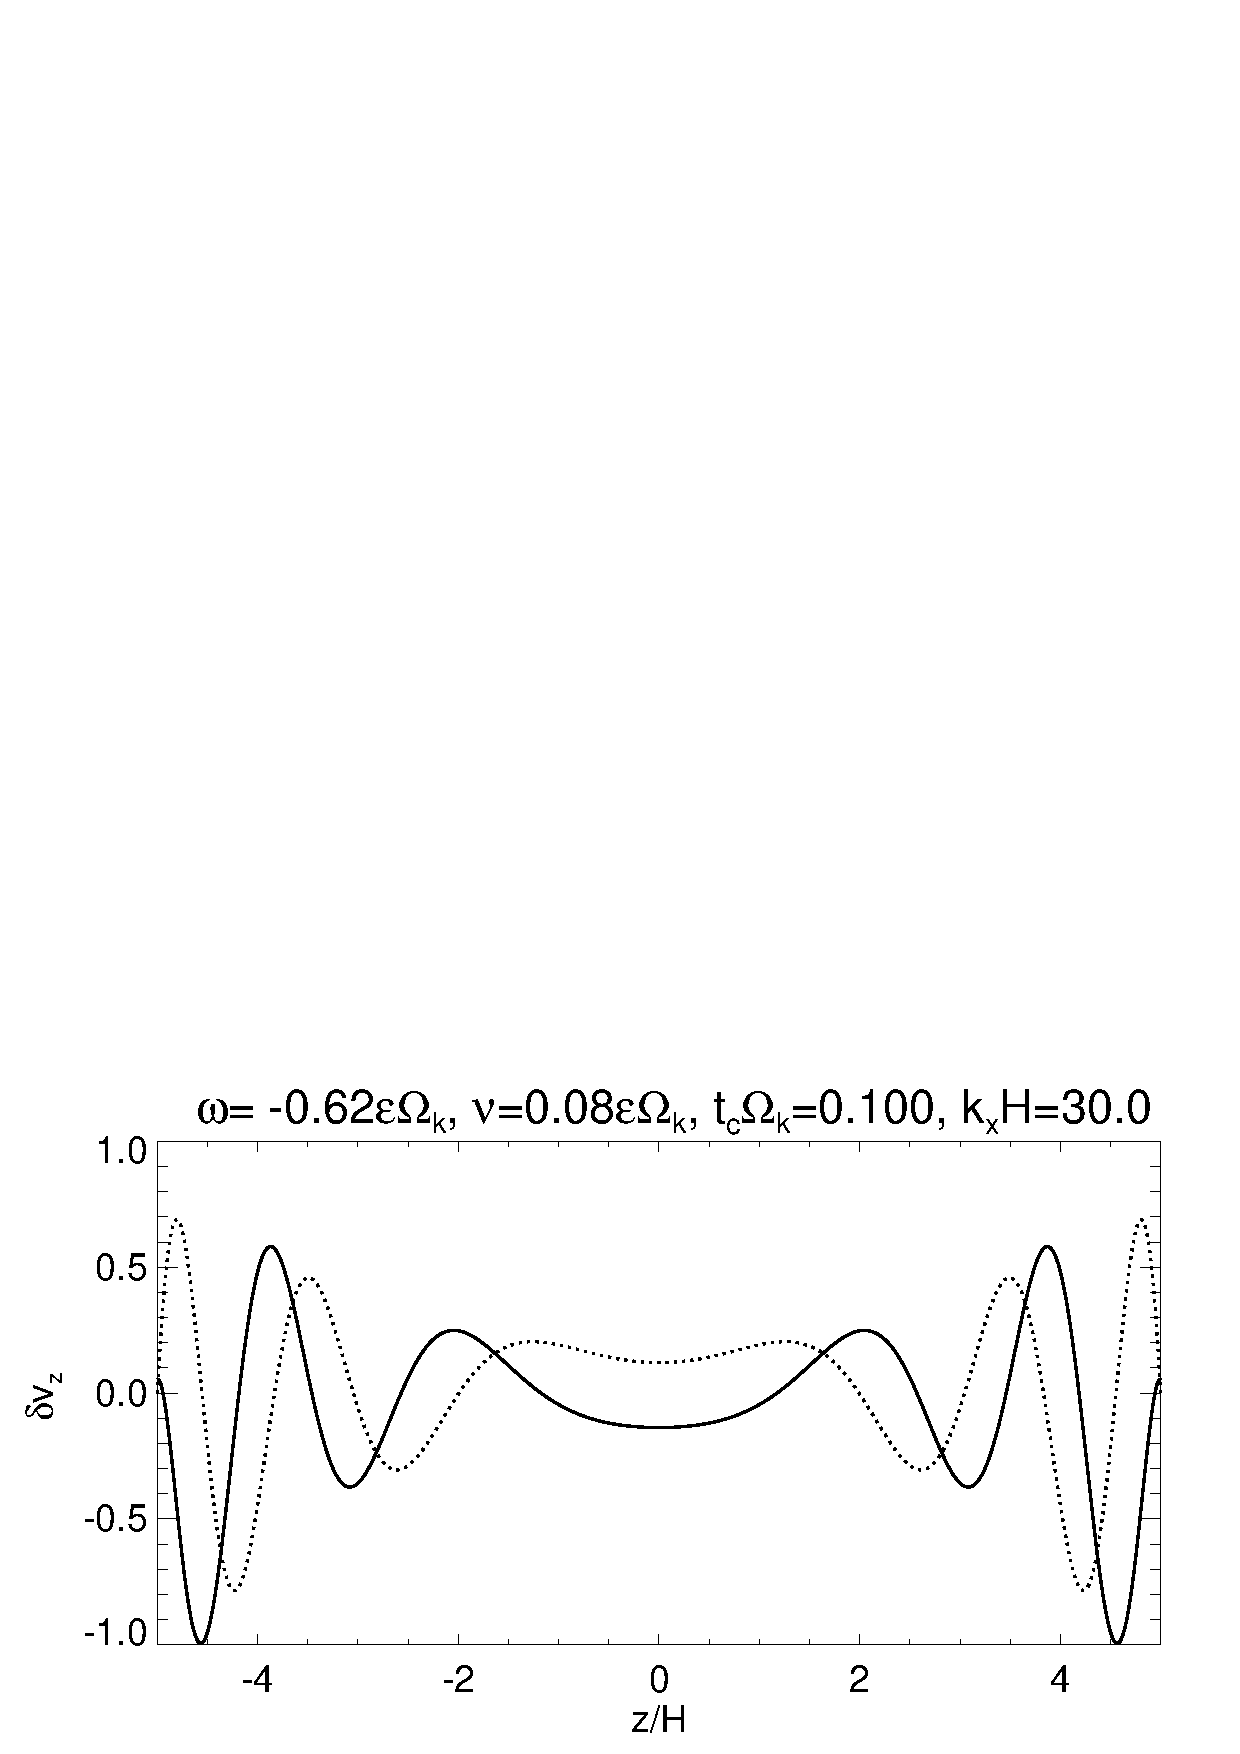
\includegraphics[width=\linewidth,clip=true,trim=0cm 0cm 0cm
  1cm]{figures/eigenvectorvz_beta0d1}
  \caption{Same as Fig. \ref{lowfreq_eigenfunc} but with a
    thermal relaxation timescale $\beta=0.1$. 
    \label{lowfreq_eigenfunc_cool}
  }
\end{figure}

\begin{figure}
  % 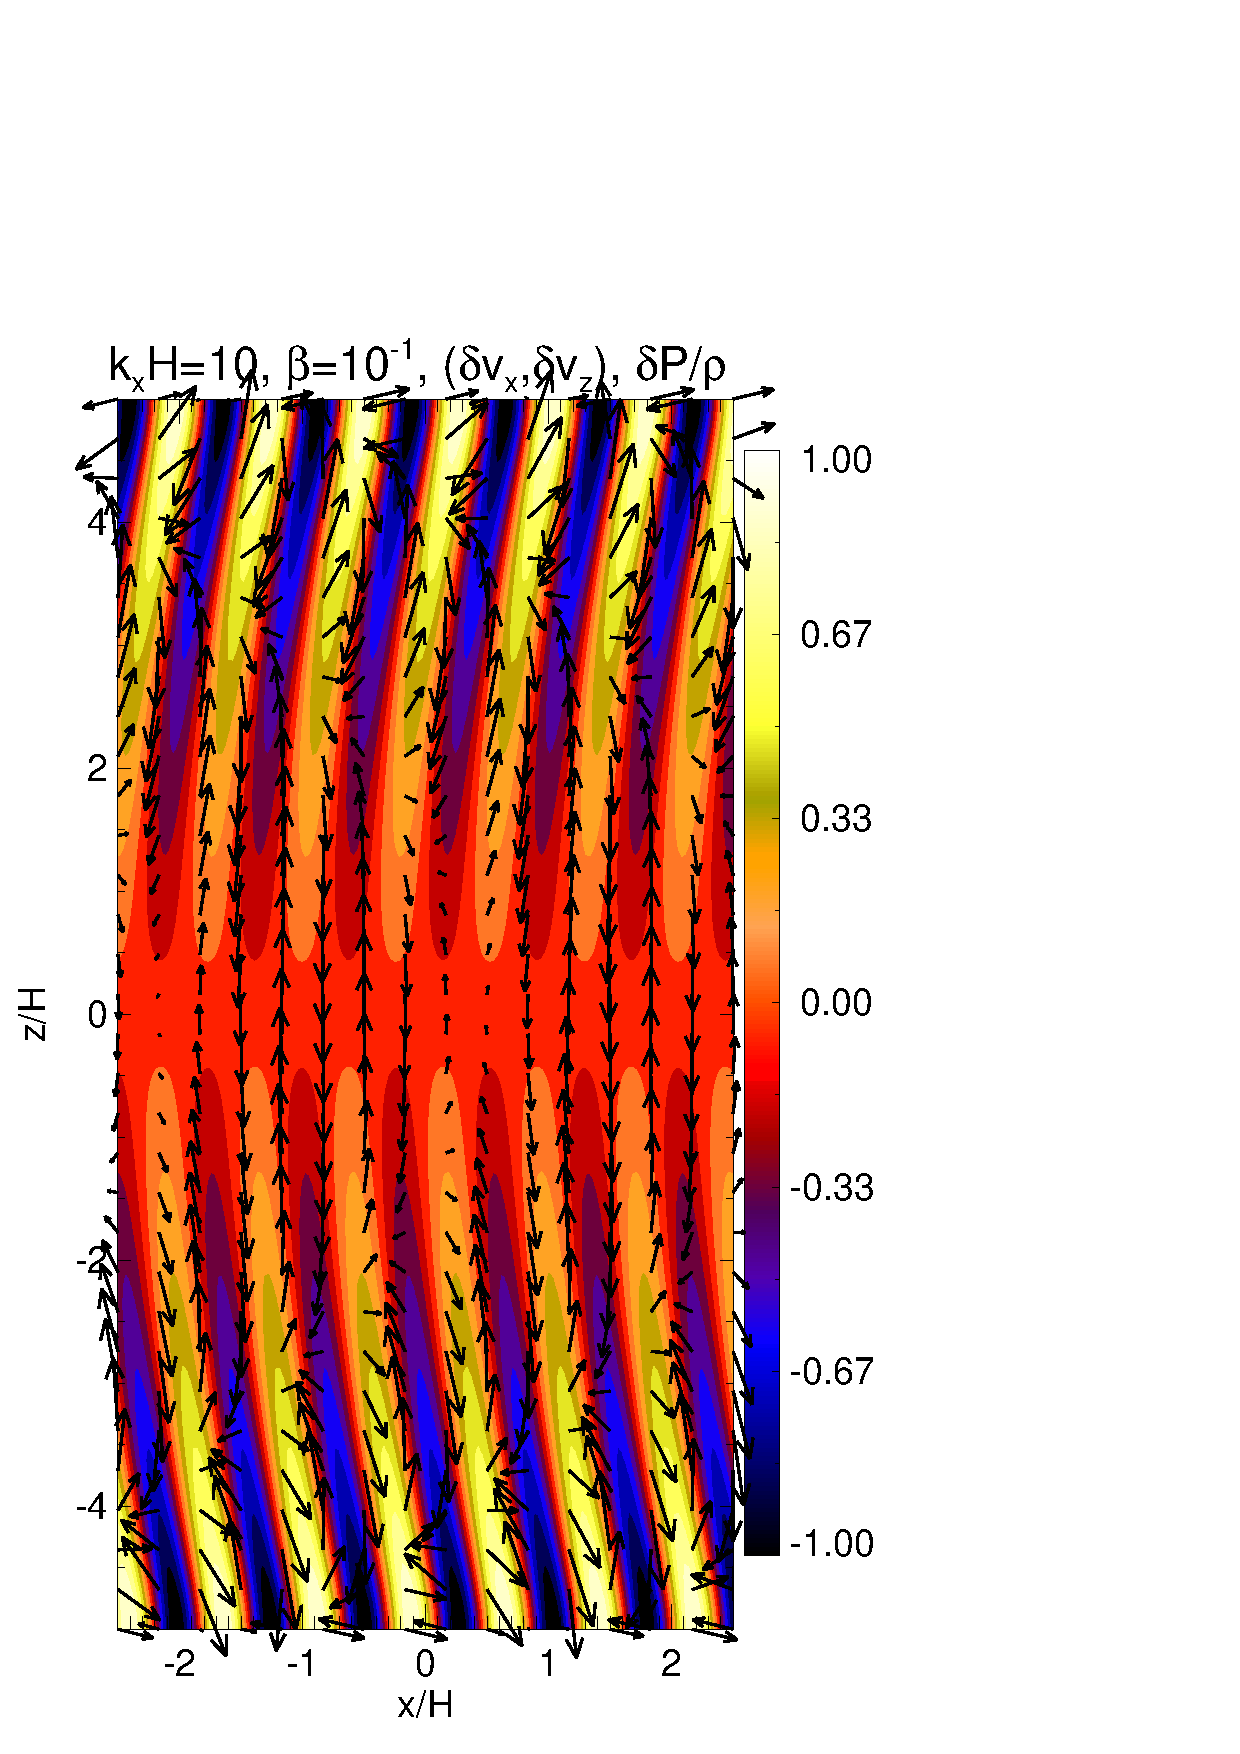
\includegraphics[scale=0.345,clip=true,trim=0cm 0cm 2.5cm
  % 0cm]{figures/result2d_vel_cool}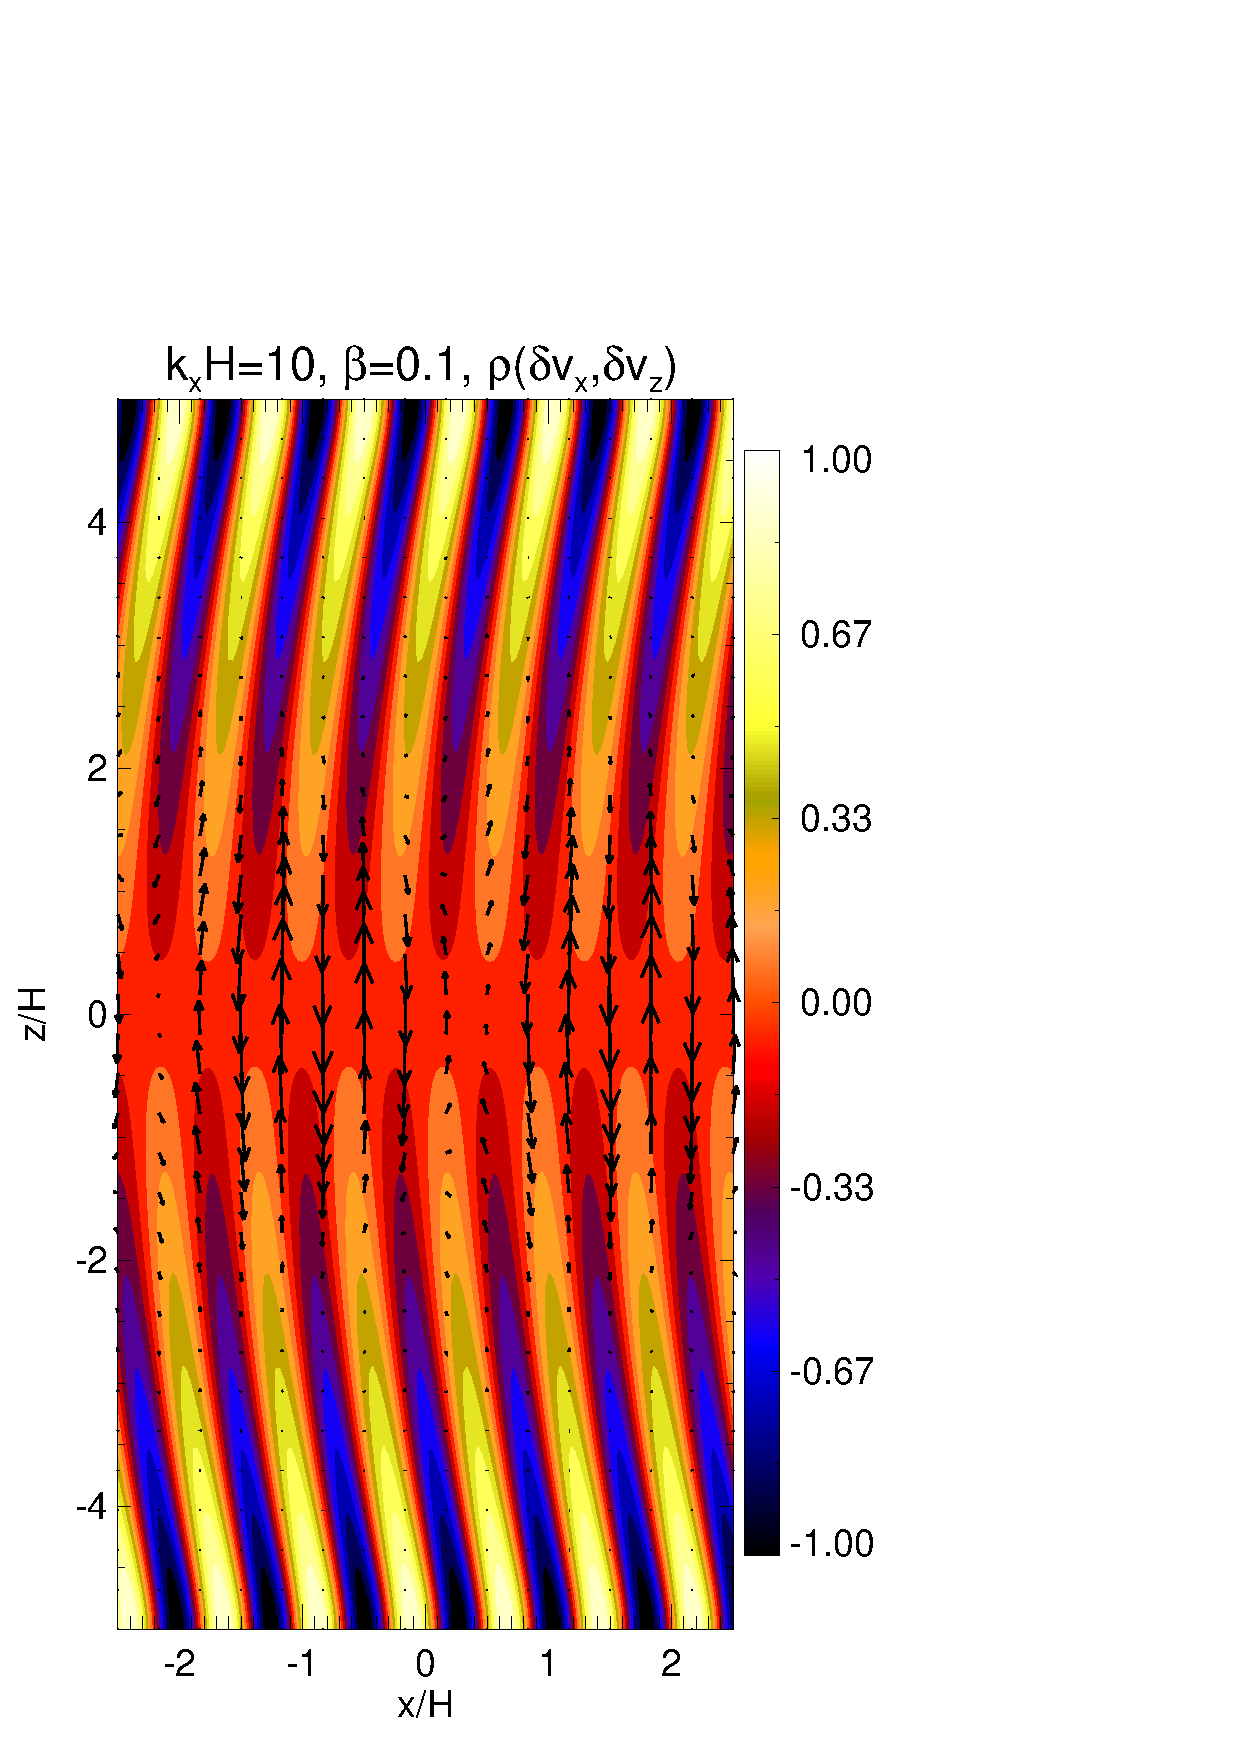
\includegraphics[scale=0.345,clip=true,trim=1.9cm 0cm 0cm
  % 0cm]{figures/result2d_mom_cool} 
  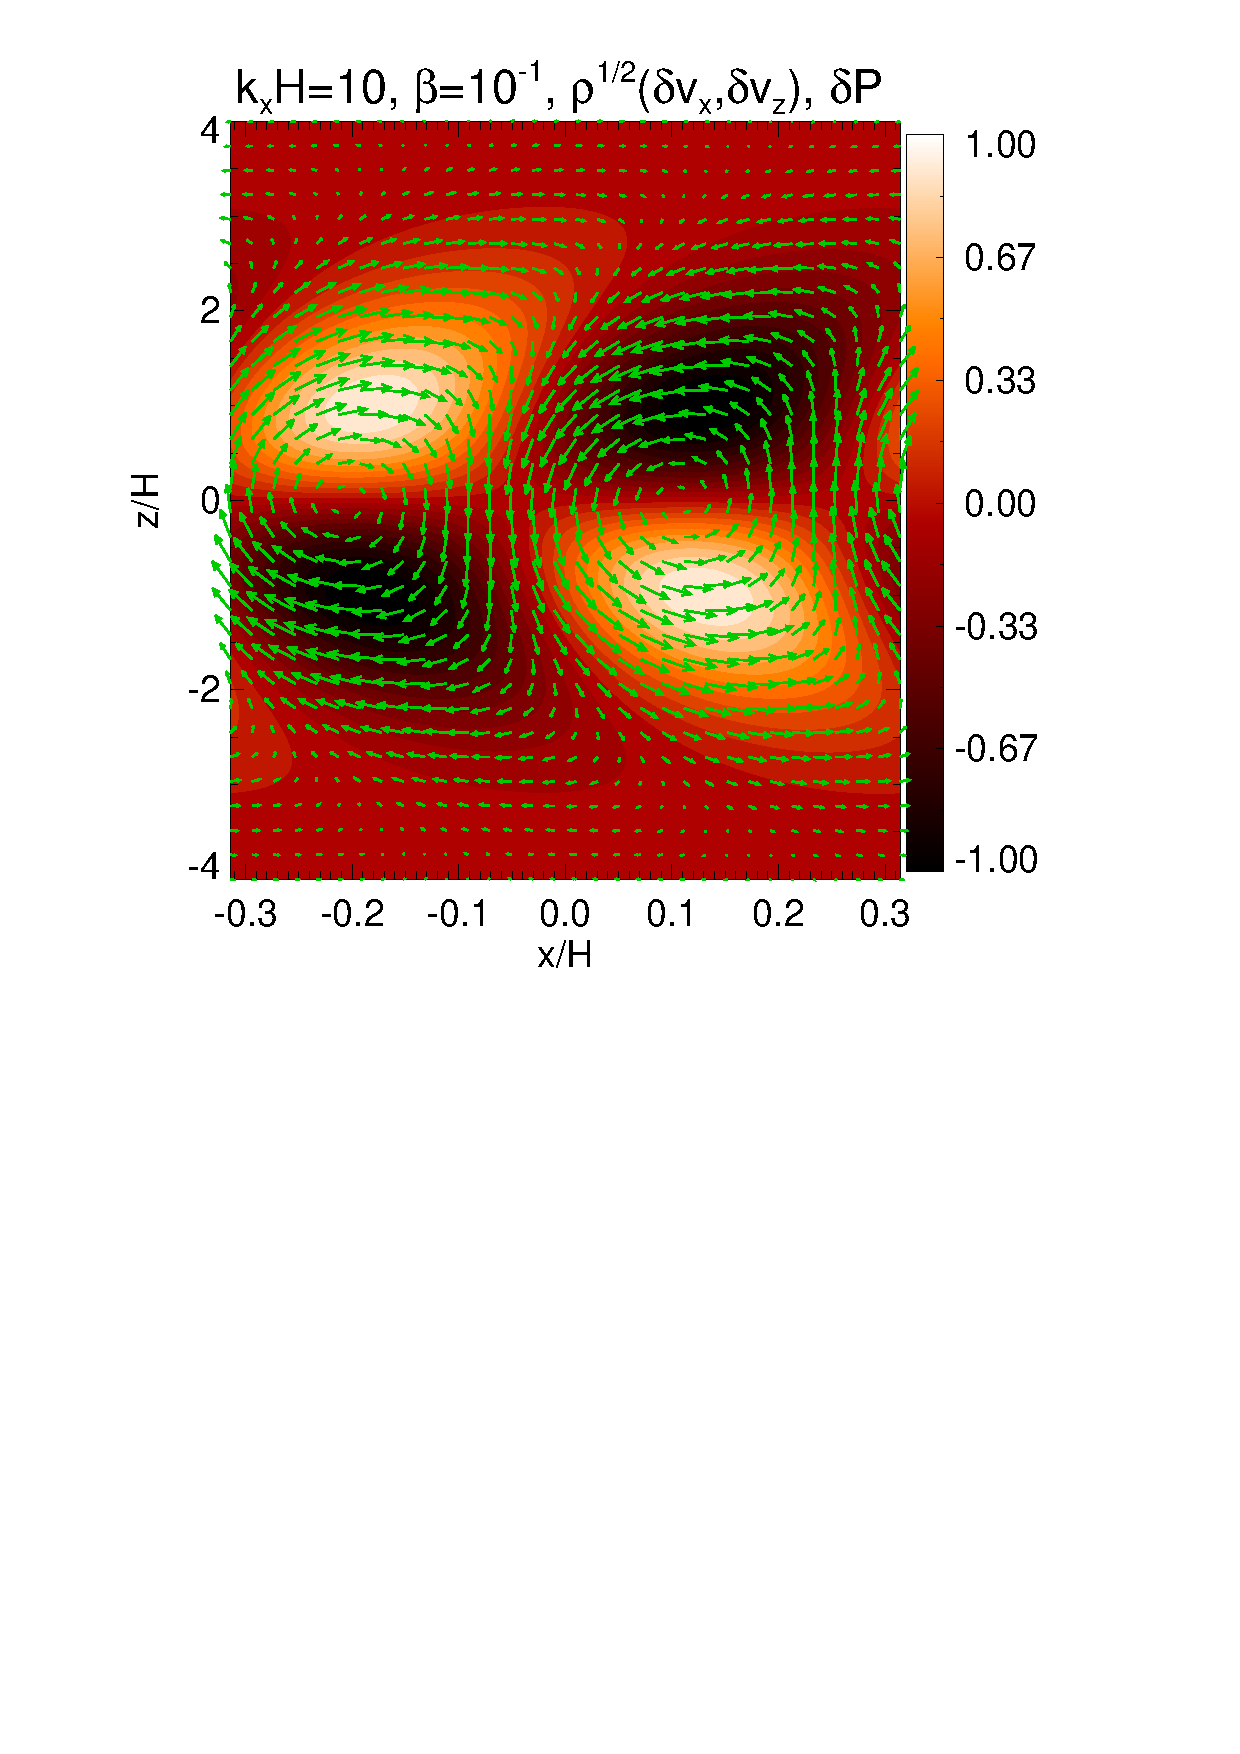
\includegraphics[width=\linewidth]{figures/result2d_cool}
  \caption{Same as  Fig. \ref{lowfreq_eigenfunc_2d} but with a thermal
    relaxation timescale $\beta=0.1$. 
    \label{lowfreq_eigenfunc_2d_cool}
  }
\end{figure}

%presence of buoyancy forces at the boundary may make BC more
%influential 

In Fig. \ref{compare_modes_cool_kx30} we plot eigenvalues for unstable 
modes with $\khat=30$. For clarity, we only plot analytic results 
for the fundamental mode ($M=0$) and $M=1,\,2$, and omit the 
squares. The fundamental mode is again insensitive to $\zmax$ and are
in close agreement with analytic results. However, 
there is increasing mismatch between analytical and numerical results
for higher order modes as $\beta$ is increased. This suggests that, in
the presence of buoyancy, boundary effects become important for these
modes, which have larger $\khat$ than that considered previously. For
example, for $\zmax=5H$ and $\zmax=7H$, we 
find modes slightly more unstable than the fundamental
mode even when $\beta=0.1$ (the leftmost eigenvalues in the lower two
panels), but these are clearly affected by boundary
conditions as they are absent for $\zmax=3H$. 

Nevertheless, as before we observe more effective stabilization for
higher order modes, including the absence of surface modes, for
example as $\beta$ is increased from $0.01$ to $0.03$ (for $\zmax\geq
5H$). If we discard modes associated with boundary conditions, then
the fundamental mode would again become the dominant mode as $\beta$ is
increased. 

\begin{figure}
  \includegraphics[width=\linewidth,clip=true,trim=0cm 1.75cm 0cm
  0cm]{figures/compare_modes_cool_kx30_z3_analytic.ps} 
  \includegraphics[width=\linewidth,clip=true,trim=0cm 1.75cm 0cm
  0cm]{figures/compare_modes_cool_kx30_z5_analytic.ps}
  \includegraphics[width=\linewidth]{figures/compare_modes_cool_kx30_z7_analytic.ps}
  \caption{Same as Fig. \ref{compare_modes_cool_kx10} but for
    $\khat=30$. Examples of surface modes are marked with `s'. 
    \label{compare_modes_cool_kx30} 
  }
\end{figure}

% Fig. \ref{compare_modes_cool_kx10} and \ref{compare_modes_cool_kx30} 
% show that the fundamental mode is not sensitive to boundary
% conditions. The fundamental mode also becomes dominant as $\beta$
% approaches $\beta_\mathrm{crit}$, except with the possible emergence
% of modes associated with boundary conditions. Thus, tracking the
% fundamental mode is a more preferable assessment of stability as $\beta$
% is increased from zero, rather than searching for the most unstable
% mode. This is because the latter may correspond to modes that depend on boundary
% conditions, e.g. surface modes whose growth rate varies with
% $\zmax$ in a vertically isothermal disk. 


%boundary conditions play an increasing role for higher M

\subsection{Critical thermal relaxation
  timescale}\label{bcrit_num_test}
In Fig. \ref{bcrit_compare1} we plot the maximum VSI growth rates
found in the fiducial disk model as a function of the thermal
relaxation timescale $\beta$ for several values of $\khat$ and
$\zmax$. We also plot the critical timescale
$\beta_\mathrm{crit}=0.125$ for the fiducial disk parameters.   

Note that the curves are not neccessarily smooth because the most unstable
mode may not always correspond to the same type of disturbance. For example,
as seen above, for $\khat \leq 10$ higher order body modes are
dominant as $\beta\to 0$, but the fundamental 
mode becomes dominant as $\beta$ is increased. For $\khat=1$ the VSI
can operate slightly beyond $\beta_\mathrm{crit}$  (recall that
$\beta_\mathrm{crit}$ was derived assuming $\khat^2\gg 1$). For
$\khat=5,\,10$ (and $30$ for $\zmax=3H$), we find
$\beta_\mathrm{crit}$ accurately predicts the thermal timescal beyond
which the VSI is suppressed.   

Complications from vertical boundaries arise when considering large
$\khat$. For $\khat=30$ and $\zmax=5H,\,7H$ we find for $\beta\gtrsim
0.1$ the dominant disturbance correspond to the leftmost eigenvalues 
seen in the lower two panels of Fig. \ref{compare_modes_cool_kx30},
which do not exist for $\zmax=3H$. For $\khat=50,\,100$ and
$\beta\to0$, we find surface modes dominate so the maximum growth rate
depends on $\zmax$ in the limit of rapid thermal relaxation. 
However, the maximum growth rate is insensitive to 
$\zmax$ for moderately large $\beta$ ($\gtrsim 0.1$), i.e. close to
the stabilization of the fundamental mode.  
%not surprising since we enable strongly stabilizing buoyancy forces
%at large zmax 

Our result is consistent with numerical simulations performed by
\citetalias{nelson13} for which a thermal relaxation timescale $\beta\gtrsim
0.6$ stabilized the VSI; as Fig. \ref{bcrit_compare1} show that growth
rates for $\beta\gtrsim 0.6$ are small, and are restricted to very
small radial lengthscales $\sim 10^{-2}H$, for which current numerical
simulations may not be able to resolve.
%  To destablize the disk with
% $\beta\gtrsim O(1)$, one might consider 
% $\khat > 100$ to increase the maximum growth rate by enabling surface
% modes, but in a realistic disk
% very small scale disturbances will likely be subject to viscous decay
% (see \S\ref{application}). 
%Numerical simulations are also unlikely to
%resolve such small scales.  

\begin{figure}
  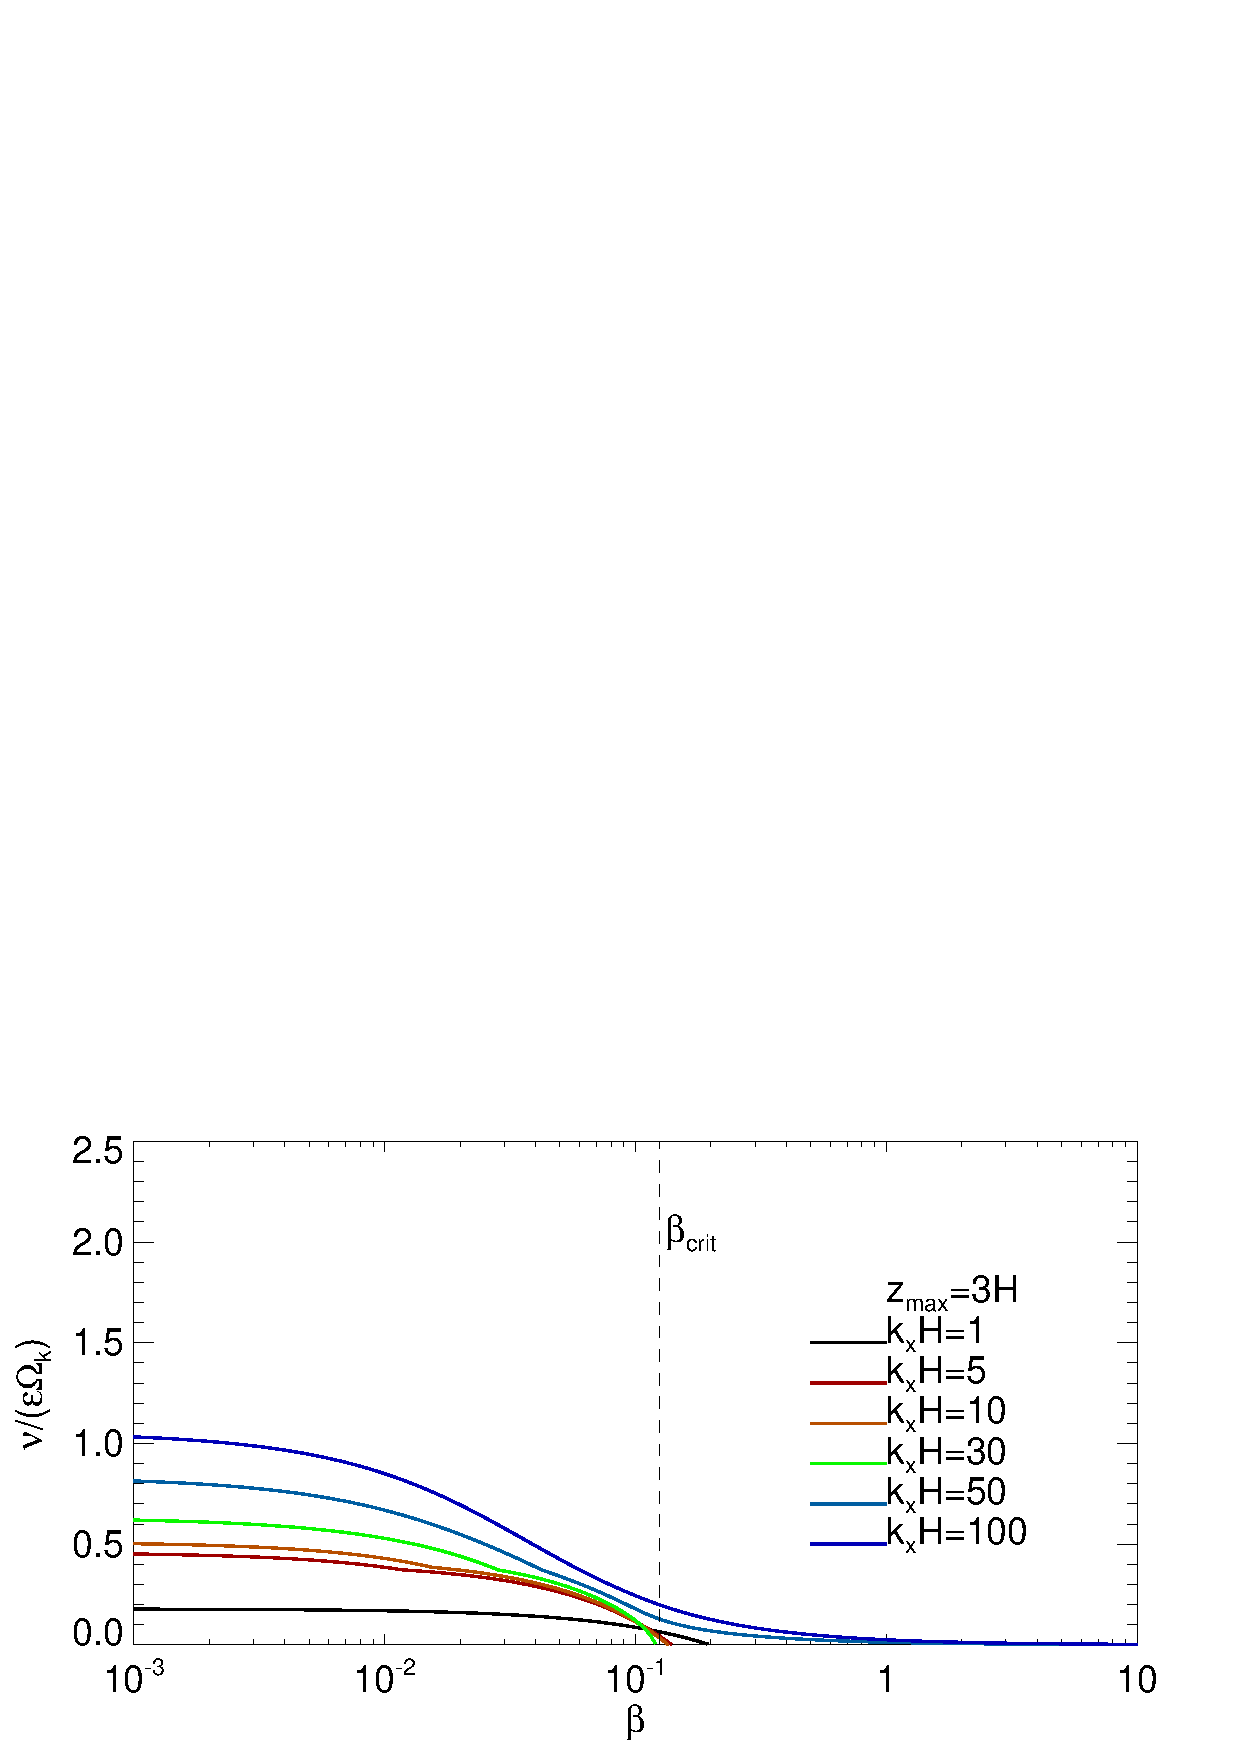
\includegraphics[width=\linewidth,clip=true,trim=0cm 1.75cm 0cm
  0.9cm]{figures/gcorr_compare_iso_maxrate_z3} 
  \includegraphics[width=\linewidth,clip=true,trim=0cm 1.75cm 0cm
  0.9cm]{figures/gcorr_compare_iso_maxrate_z5} 
  \includegraphics[width=\linewidth,clip=true,trim=0cm 0.0cm 0cm
  0.9cm]{figures/gcorr_compare_iso_maxrate_z7}  
  \caption{Maximum VSI growth rates in the fiducial disk 
     model as a function of the thermal relaxation timescale
     $\beta$, for $\zmax=3H$ (top), $\zmax=5H$ (middle, standard
     setup) and $\zmax=7H$ (bottom). The vertical line is the
     critical thermal timescale $\beta_\mathrm{crit}$ obtained  
     from Eq. \ref{iso_vsi_cond}. 
     \label{bcrit_compare1}}   
 \end{figure} 

As pointed out by \citetalias{barker15}, in vertically isothermal disks with
an imposed boundary, surface modes are dependent on $\zmax$, but they
are often the most unstable. Despite this caveat, and that surface
modes are not accounted in our analysis, we see from
Fig. \ref{bcrit_compare1} that $\beta_\mathrm{crit}$ nevertheless
provides a reasonable estimate for an upper limit to the thermal
timescale for the VSI.  
%It becomes an accurate criter when considering fixed
%$\khat$  

We further  test the dependence of $\beta_\mathrm{crit}$ on disk parameters
(Eq. \ref{iso_vsi_cond}).  We use the fiducial setup as a  reference
point and vary $q\in[-0.2,-1.2]$,  $\gamma\in[1.2,2.0]$, and
$ h\in[0.02,0.1]$ separately. The numerically obtained
$\beta_\mathrm{crit}$ are shown in Fig. \ref{bcrit_compare} in
comparison with Eq. \ref{iso_vsi_cond}, which generally agree. This
result, together with Fig. \ref{bcrit_compare1}, shows that  
$\beta \lesssim \beta_\mathrm{crit}$ is a practical
criteria for the VSI to operate effectively in stably stratified,
vertically isothermal disks.   

% The agreement improves with decreasing  $|q|$,
% $ h$ and increasing $\gamma$, i.e. weaker instability. There is
% a noticeable difference as $\gamma\to1$ because the derivation of
% $\beta_\mathrm{crit}$ assumed $\gamma>1$. 

\begin{figure}
  \includegraphics[width=\linewidth,clip=true,trim=0cm 0.cm 0cm
  0cm]{figures/bcrit_compare_q.ps} 
  \includegraphics[width=\linewidth,clip=true,trim=0cm 0.0cm 0cm
  0.8cm]{figures/bcrit_compare_g.ps}
  \includegraphics[width=\linewidth,clip=true,trim=0cm 0.0cm 0cm
  0.8cm]{figures/bcrit_compare_e.ps} 
  \caption{Dependence of the upper limit to the thermal relaxation timescale
    $\beta_\mathrm{crit}$ for the fundamental VSI mode on disk
    parameters. The fiducial setup is $(\gamma, \Gamma= (1.4, 1.011)$
    and $(p,q, h)=(-1.5,-1,0.05)$. Top: varying 
    $q\in[-1.2,-0.2]$; middle: varying $\gamma\in[1.2,2.0]$; bottom:
    varying $ h\in[0.02,0.1]$. The perturbation wavenumber is
    $\khat=10$.  
    \label{bcrit_compare}}  
\end{figure}

\subsection{Vertically non-isothermal disk model} 
%We briefly consider vertically non-isothermal disks in which there is
%a disk surface at finite height. 
\citetalias{barker15} have argued that vertically isothermal disks are not
ideal for studing the VSI because $\zmax$ is a free 
parameter in numerical calcluations. On the other hand, vertically 
non-isothermal disks have a disk surface at finite height so there is
a natural choice for $\zmax$. This means that higher order body modes and
surface modes are better defined in a vertically non-isothermal disk.   

However, as we have seen in Fig. \ref{bcrit_compare1}, the maximum
growth rate becomes insensitive to $\zmax$ for $\beta\gtrsim
\beta_\mathrm{crit}$. This suggests that the characteristic upper
limit on the thermal timescale for the VSI is not sensitive to
$\zmax$, so that vertically isothermal disks are in fact suitable for
the purpose of this paper. 

%Physically this is because modes that depend on vertical boundaries
%are also subject to the strongest stabilization by buoyancy, which
%maximize at $\zmax$. These modes are theremore always strongly damped
%as we increase the thermal timescale. 

Nevertheless, here we briefly consider a vertically non-isothermal
disk model with $(p,q, h)=(0,-1,0.05)$ and $\Gamma=1.0837$. This
value of $\Gamma$ is chosen so that the standard vertical domain size $\zmax =
5H$ effectively corresponds to the disk surface ($\zmax\simeq
H_s$). The disk temperature decreases rapidly with height such that 
$c_s^2(\zmax)\simeq 10^{-4}c_s^2(0)$.    

In Fig. \ref{compare_modes_vnoniso_kx10} we plot the mode diagram for
$\khat=10$ for several values of $\beta$. This plot is 
qualitatively similar to Fig. \ref{compare_modes_cool_kx10}. As before
we find as $\beta$ is increased, higher order body modes are rapidly
stabilized, eventually only the fundamental mode can operate before
the VSI is entirely suppressed.  

\begin{figure}
  \includegraphics[width=\linewidth,clip=true,trim=0cm 0cm 0cm
  0cm]{figures/compare_modes_Gam1.084_kx10.ps}
  \caption{Unstable modes in a vertically non-isothermal disk with
    $\khat=10$ and a range of thermal relaxation timescales.  
    \label{compare_modes_vnoniso_kx10}}
\end{figure}

We do not find surface modes for $\khat=10$, but do find them for
sufficiently large $\khat$. We demonstrate this in  % In the vertically
% non-isothermal disk, surface modes develop for sufficiently large 
% $\khat$ \citep{barker15}. We demonstrate them in
Fig. \ref{compare_modes_vnoniso_kx100} which show eigenvalues for
$\khat=100$. While growth rates generally decrease with increasing 
$\beta$, we find eigenvalues can overlap, making it difficult to 
distinguish between different modes. However, since there 
is a well-defined surface, we may seek the  
most unstable mode without the boundary-dependent issue that arose 
with a vertically isothermal disk in the limit $\beta\to0$.  

\begin{figure}
  \includegraphics[width=\linewidth,clip=true,trim=0cm 0cm 0cm
  0cm]{figures/compare_modes_Gam1.084_kx100.ps}
  \caption{Same as Fig. \ref{compare_modes_vnoniso_kx10} but with
    $\khat=100$. In this case surface modes appear nearly parallel to
    the vertical axis
    (cf. Fig. \ref{compare_modes_vnoniso_kx10}). However, this
    distinction becomes difficult for increasing $\beta$ as modes
    overlap. 
    % but
    % overlap with body modes (those that are roughly horizontal when 
    % $\beta=10^{-3}$) as $\beta$ is further increased. 
    \label{compare_modes_vnoniso_kx100}}
\end{figure}

Fig. \ref{compare_eigenvz_vnoniso_kx100} show the most unstable modes
with $\khat=100$ and $\beta=10^{-3},\, 10^{-2}$ and
$0.1$. For $\beta=10^{-3}$ the most 
unstable mode is an asymmetric surface mode \citepalias[also seen in Fig. 7
of][]{barker15}. However, increasing the thermal timescale to
$\beta=10^{-2}$ an anti-symmetric surface mode becomes
dominant. Further increasing to $\beta=0.1$, the dominant mode has a
mixed character between a surface mode and the fundamental
mode. Notice as $\beta$ is increased the perturbation amplitude near
the vertical boundaries become negligible. This is not surprsing since  
the stabilizing effect of buoyancy is largest at the disk surface. 
%formally diverges 

\begin{figure}
  \includegraphics[width=\linewidth,clip=true,trim=0cm 1.73cm 0cm
  0cm]{figures/eigenvectorvz_vnoniso_kx100_beta0d001.ps}
  \includegraphics[width=\linewidth,clip=true,trim=0cm 1.73cm 0cm
  0cm]{figures/eigenvectorvz_vnoniso_kx100_beta0d01.ps}
  \includegraphics[width=\linewidth,clip=true,trim=0cm 0cm 0cm
  0cm]{figures/eigenvectorvz_vnoniso_kx100_beta0d1.ps}
  \caption{Vertical velocity eigenfunction of the most unstable mode
    with $\khat=100$ found in the vertically non-isothermal disk with
    $\beta = 10^{-3}$ (top), $\beta=10^{-2}$ (middle) and $\beta=0.1$
    (bottom). 
    \label{compare_eigenvz_vnoniso_kx100}}
\end{figure}
  
Finally, in Fig. \ref{bcrit_compare2} we plot the maximum VSI growth
rates in the vertically non-isothermal disk model. Based on 
Eq. \ref{iso_vsi_cond}, we conjecture the critical 
thermal timescale in the vertically non-isothermal disk is 
given by $ h|s|/(\gamma - \Gamma)$. This 
evaluates to 0.158, which is close to the cut-off thermal timescale
for $\khat\in[5,30]$. Fig. \ref{bcrit_compare2} is qualitatively 
similar to the fiducial disk model in
Fig. \ref{bcrit_compare1}. Importantly, for $\khat=O(10)$ there is a
precise cut-off thermal timescale, the value of which in fact provides a  
characteristic upper limit for other $\khat$. 

\begin{figure}
  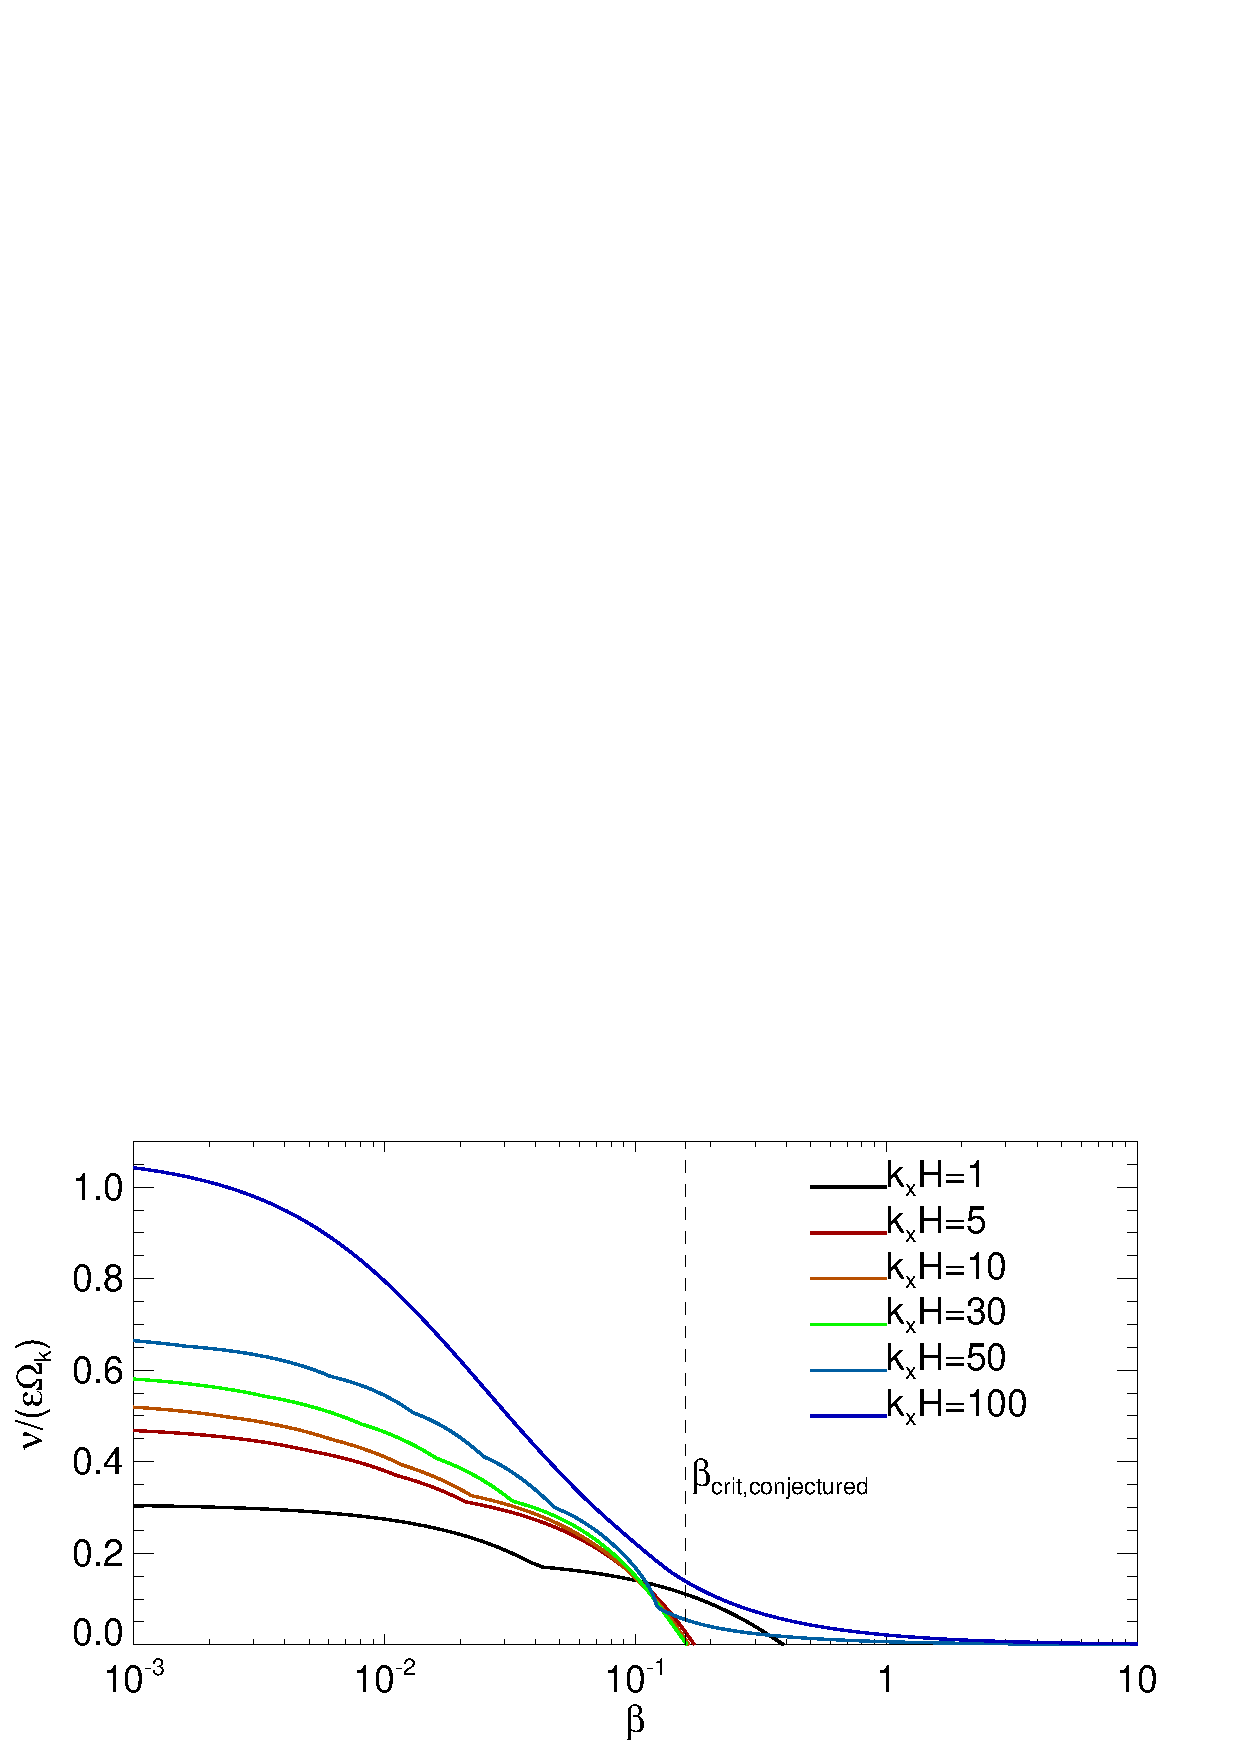
\includegraphics[width=\linewidth]{figures/gcorr_compare_vnoniso_maxrate} 
  \caption{Maximum VSI growth rates in the vertically non-isothermal disk
    model as a function of the thermal relaxation timescale
    $\beta$. The vertical line is a conjectured 
    critical thermal timescale given by
    $ h|s|/(\gamma-\Gamma)=0.158$.  
    \label{bcrit_compare2}}   
\end{figure} 


  % We briefly consider vertically non-isothermal disks with 
% $\Gamma=1.4$ and $(p,q, h)=(0,-1,0.05)$ as simulated in
% \cite{nelson13}. In this case we set $\zmax=0.99H_s$.  

% Fig. \ref{gcorr_compare_vnoniso} plots the fundamental VSI growth
% rates as a function of $\beta$ for $\gamma\in[1.4,2.5]$. In agreement
% with \citeauthor{nelson13}, in   
% the neutrally-stratified case $\gamma=\Gamma$ the disk is unstable 
% even for $\beta\gg 1$. This is due to the absence of a stabilizing
% vertical entropy gradient ($N_z^2\equiv 0$). % (Note that in the adiabatic limit 
% % this disk can be unstable according to the
% % Solberg-Hoiland criterion, Eq. \ref{solberg2}.) 

% For $\gamma>\Gamma$, i.e. stably stratified disks,
% Fig. \ref{gcorr_compare_vnoniso} shows that introducing finite thermal
% relaxation rapidly stabilizes the disk, similar to that observed for
% nearly vertically isothermal disks (Fig. \ref{bcrit_compare1}). For
% $\gamma=1.7,\,2.0,\,2.5$, growth rates reach zero at
% $\beta\simeq0.17,\,0.083,\,0.045$, respectively. Interestingly, these
% values are equal to $ h|q|/(\gamma-\Gamma)$. This suggests that
% the critical thermal relaxation timescale for vertically
% non-isothermal disks can also be estimated by Eq. \ref{iso_vsi_cond}
% but with $\gamma-1$ replaced by $\gamma-\Gamma$. 

% \begin{figure}
%   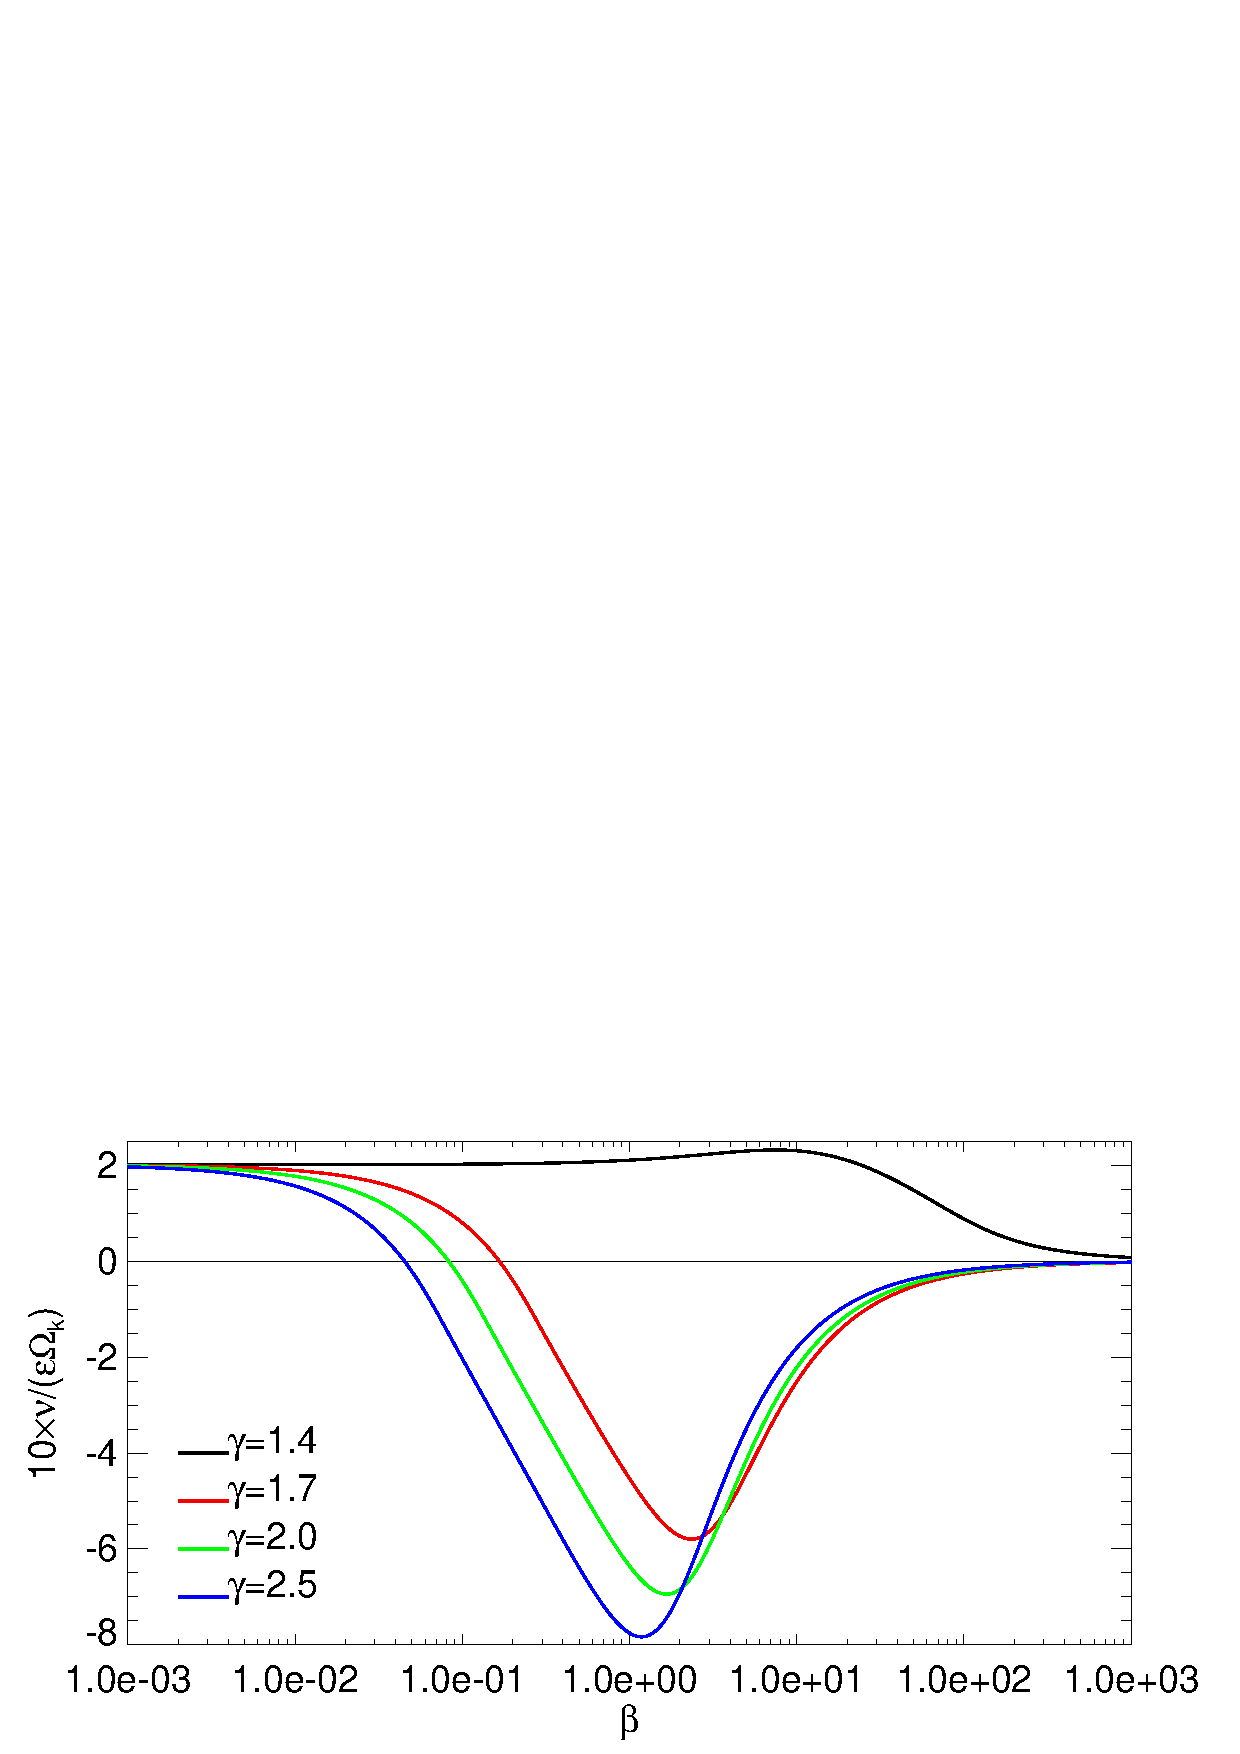
\includegraphics[width=\linewidth,clip=true,trim=0cm 0cm 0cm
%   0cm]{figures/gcorr_compare_vnoniso2}
%   \caption{Growth rate of the fundamental VSI mode as a function of
%     the thermal relaxation timescale $\beta$, in vertically
%     non-isothermal disks with $\Gamma=1.4$ and
%     $\gamma\in[1.4,2.5]$. The disk is neutrally
%     stratified for $\gamma=1.4$ and stably stratified for
%     $\gamma>1.4$. Other disk parameters are
%     $(p,q, h)=(0,-1,0.05)$ and the perturbation wavenumber is
%     $\khat=30$.   
%     \label{gcorr_compare_vnoniso}}
% \end{figure}












